\documentclass[11 pt, oneside]{book} %oneside

\usepackage{amsmath, amsthm, amssymb, mathrsfs}
\usepackage{graphicx}
\usepackage{cite}
\usepackage[left=1.5in,top=1in,right=1in,nohead,foot=1in]{geometry}
\usepackage{fancyhdr}

\bibliographystyle{ieeetr} 
\pagestyle{plain}%headings, myheadings, fancy

\renewcommand{\v}[1]{\ensuremath{\mathbf{#1}}} % for vectors
\newcommand{\gv}[1]{\ensuremath{\mbox{\boldmath$ #1 $}}} 
% for vectors of Greek letters
\newcommand{\uv}[1]{\ensuremath{\mathbf{\hat{#1}}}} % for unit vector
\newcommand{\abs}[1]{\left| #1 \right|} % for absolute value
\newcommand{\avg}[1]{\left< #1 \right>} % for average
\let\underdot=\d % rename builtin command \d{} to \underdot{}
\renewcommand{\d}[2]{\frac{d #1}{d #2}} % for derivatives
\newcommand{\dd}[2]{\frac{d^2 #1}{d #2^2}} % for double derivatives
\newcommand{\pd}[2]{\frac{\partial #1}{\partial #2}} 
% for partial derivatives
\newcommand{\pdd}[2]{\frac{\partial^2 #1}{\partial #2^2}} 
% for double partial derivatives
\newcommand{\pdc}[3]{\left( \frac{\partial #1}{\partial #2}
 \right)_{#3}} % for thermodynamic partial derivatives
\newcommand{\ket}[1]{\left| #1 \right>} % for Dirac bras
\newcommand{\bra}[1]{\left< #1 \right|} % for Dirac kets
\newcommand{\braket}[2]{\left< #1 \vphantom{#2} \right|
 \left. #2 \vphantom{#1} \right>} % for Dirac brackets
\newcommand{\matrixel}[3]{\left< #1 \vphantom{#2#3} \right|
 #2 \left| #3 \vphantom{#1#2} \right>} % for Dirac matrix elements
\newcommand{\grad}[1]{\gv{\nabla} #1} % for gradient
\let\divsymb=\div % rename builtin command \div to \divsymb
\renewcommand{\div}[1]{\gv{\nabla} \cdot #1} % for divergence
\newcommand{\curl}[1]{\gv{\nabla} \times #1} % for curl

% ABSTRACT

\newenvironment{abstract}
{\thispagestyle{empty}
\begin{center}
\vspace*{1.5cm}
{\Large \bfseries Abstract}
\end{center}
\vspace{0.5cm}
\begin{quote}}
{\end{quote}}

% DEDICATION
%
% The dedication environment makes sure the dedication gets its
% own page and is set out in verse format.

\newenvironment{dedication}
{\thispagestyle{empty}
  \begin{center}
  \vspace*{1.5cm}
  {\LARGE }
  \end{center}
  \vspace{0.5cm}
  \begin{verse}\begin{center}}
{\end{center}\end{verse}}


% ACKNOWLEDGEMENTS
%
% The acknowledgements environment puts a large, bold, centered 
% "Acknowledgements" label at the top of the page. The acknowledgements
% themselves appear in a quote environment, i.e. tabbed in at both sides, and
% on its own page.

\newenvironment{acknowledgements}
{\thispagestyle{empty}
\begin{center}
\vspace*{1.5cm}
{\Large \bfseries Acknowledgements}
\end{center}
\vspace{0.5cm}
}
%\begin{quote}}
%{\end{quote}}

\begin{document}
\title{Circuit QED with Highly Multimodal Photon-Qubit Strong Coupling}

\author{Alexander Pease \\
\texttt{apease@princeton.edu}\\
\\
Advisor: Andrew Houck\\
\\
A Thesis presented to the\\ 
Department of Physics of
Princeton University\\
in Candidacy for the Degree of \\
Bachelor of Arts\\
\\
\\}

\date{May 7th, 2012}
\maketitle

%%%%%%%%%%%%%%%%%
\begin{center}
This paper represents my own work in accordance with University regulations. \par
\vspace{1.5cm}
\hspace{0.5cm} \makebox[3.5in]{\hrulefill}\\
Alexander Pease
\end{center}

%%%%%%%%%%%%%%%%%
\newpage
\begin{abstract}
Text here
\end{abstract}


%: ----------------------- contents ------------------------

\setcounter{secnumdepth}{3} % organisational level that receives a numbers
\setcounter{tocdepth}{3}    % print table of contents for level 3
\tableofcontents            % print the table of contents
% levels are: 0 - chapter, 1 - section, 2 - subsection, 3 - subsection


%: ----------------------- list of figures/tables ------------------------

\listoffigures	% print list of figures

\listoftables  % print list of tables


%%%%%%%%%%%%%%%%%
\newpage
\begin{dedication}
\emph{For my grandfather,\\Without your genes, this never would have happened}
\end{dedication}

%%%%%%%%%%%%%%%%%
\newpage
\begin{acknowledgements}
I would first like to thank my advisor Andrew Houck, who makes me question the horror stories I so frequently hear about inaccessible, aloof advisors. 

However, I feel most indebted to Devon Underwood, who was infinitely patient with me. Laboratory work is a long and complex process and, even after initially teaching me everything, Devon would always help once I had already made every conceivable mistake. 

To Srikanth Srinivasan, who graciously offered his time and electron beam lithography skills to help fabricate transmon qubits. And to all the other members of Andrew's lab, for helping me along in each and every way. 

None of the experimental work would have been possible without the resources and staff of the Micro-/Nanofabrication Laboratory. It is easy to forget how much work goes into maintaining a laboratory, without which none of the E-Quad $4^{\mathrm{th}}$ floor would have anything to do. 

To Tower Club, for being my home here at Princeton, although I hate you all for having earlier thesis due dates than me.

And of course to my family, for having no idea what I'm doing yet still providing love and encouragement just the same. 
\end{acknowledgements}

%%%%%%%%%%%%%%%%%%%%%%%%%%%%%%%%%%%%%%%%%%%%%%%%%%%%%%%%%%%%%%%%%%%%%%%
%%%%%%%%%%%%%%%%%%%%%%%%%%%%%%%%%%%%%%%%%%%%%%%%%%%%%%%%%%%%%%%%%%%%%%%
%%%%%%%%%%%%%%%%%%%%%%%%%%%%%%%%%%%%%%%%%%%%%%%%%%%%%%%%%%%%%%%%%%%%%%%
%%%%%%%%%%%%%%%%%%%%%%%%%%%%%%%%%%%%%%%%%%%%%%%%%%%%%%%%%%%%%%%%%%%%%%%
%%%%%%%%%%%%%%%%%%%%%%%%%%%%%%%%%%%%%%%%%%%%%%%%%%%%%%%%%%%%%%%%%%%%%%%
\chapter{Introduction}\label{chap:Introduction}
%We live in a world of information. Information is the fuel driving every facet of our society; from our daily email exchanges to the global economy to the DNA of every living organism, we are comfortable in our understanding that information is of fundamental importance. We are perhaps most familiar with a mathematical definition of the ``bit"- a binary digit, zero or one, the basis of all logical computation. 

%We live in a world of information. Information is the fuel driving every facet of our lives, from our daily email exchanges to the global economy to the DNA the makes us unique. And yet we tend to consider information in simplistic terms. The ``bit" - a binary digit, zero or one, the basis of all logical computation - is an absolute idea. Perceived as being the fundamental unit of information, John Wheeler once described Nature as ``it from bit."

We live in a world of information. It is the fuel driving every aspect of our lives, from our daily email exchanges to the global economy to the DNA that makes us unique. In all of this, it is easy to overlook that information is an inherently physical quantity. 

Current technology rests upon the ``bit" - a binary digit, zero or one, the basis of all logical computation. This may be a voltage level in a circuit, a polarization state, or any other such well-defined two-level system. Perceived as being the fundamental unit of information, John Wheeler once described Nature as ``it from bit."

This conception of information is fundamentally wrong, or at least incomplete. Since the rise of quantum mechanics at the beginning of the 20$^{\mathrm{th}}$ century, physicists have understood that we live in a world of inherent randomness and non-locality. At the smallest levels of matter, there is no such thing as a bit. Rather, we have co-opted numerous physical structures to \emph{represent} a perfect binary system; a bit of just a single volt is made up of 10$^{19}$ electrons! And so, as physicists are wont to do, Richard Feynman posed a difficult question: ``What is information in a quantum mechanical world?" 

The field of quantum computing not only seeks to answer this question but to control quantum information for practical purposes. This has been motivated by theoretical work realizing that quantum systems could provide major advances in computational power. A quantum computer implementing Shor's algorithm\cite{Shor}, for instance, would exponentially outperform a digital computer in factoring large integers, such as those used in Rivest-Shamir-Adelman (RSA) encryption. Similarly, the Grover search algorithm\cite{Grover} provides quadratic improvement over classical methods for searching unstructured data.

Research into quantum computing has utilized numerous viable architectures. This thesis seeks to contribute to our understanding of just one such implementation, circuit quantum electrodynamics. The underlying science of this field draws upon the existing literature of cavity quantum electrodynamics. This introduction will give a brief overview into both fields. 



%introduce other branches of quantum computing, then focus on cQED and it's origins in cavity QED
%\cite{LossDiVincenzo} first electron spin proposal

%Factor large numbers /cite{}, simulate quantum physics /cite{}. Shore and Grover’s algorithms.  RSA?
%Exponential parallel processing by quantum mechanics
%Compare to binary bits…n qubits can be in a superposition of 2^n basis states. Applying a single operation simultaneously computes output for all 2^n inputs. 
%Information is inherently a physical quantity, and the physics of information is the physics of all matter [Landauer1991]

\section{Cavity quantum electrodynamics}
Cavity quantum electrodynamics (cavity QED or CQED) is the study of the interaction between light and matter at the quantum level. Despite being wave-like in nature, electromagnetic fields are composed of discrete packets known as photons. This quantization, rather than being a matter of bookkeeping, has subtle and far reaching effects \cite{Schuster}. Amazingly, wave-like behavior is not just an emergent phenomenon arising from millions of photonic constituents; even a single photon displays a wave-particle duality. 

Consider a single photon inside of a confined cavity. Classically, the walls of the cavity act as mirrors reflecting the photon back and forth as many as one million times \cite{Vahala}. Quantum mechanically, this system is ideal for considering a very subtle question: ``What is the shape of a photon?" Both the spatial and temporal distributions of energy are not fixed, but are dependent and \emph{controllable} by the boundary conditions imposed upon the photon by matter \cite{Schuster}. By engineering a cavity, we can control the physical properties of quantized electromagnetic radiation. 

The simplest CQED system places an atom inside this same cavity. Coupled to an atomic system, a photon is no longer simply oscillating in the cavity. The two subsystems may interact, transferring energy, even destroying the photon (a non-conserved bosonic particle). The atom may be excited into a higher energy state, eventually decaying back down via spontaneous emission. Remarkably, the existence of the cavity also controls the behavior of the atom in this regard, affecting the rates of decay for various frequencies do not ``fit" inside the cavity. An atom has a higher rate of decay for frequencies that match the resonant frequency of the cavity. This enhancement is described by the Purcell factor \cite{Purcell},

\begin{equation}
F_P=\frac{3}{4\pi^2}\left(\frac{\lambda_c}{n}\right)^3\left(\frac{Q}{V}\right)
\end{equation}

for which $\lambda_c/n$ is the emitted wavelength and $Q$ and $V$ are the quality factor and mode volume of the cavity, respectively. In short, cavity QED allows one to suppress, enhance, and even make coherent the radiative decay of an atom.

Remarkably, the cavity itself (a macroscopic system!) is also affected quantum mechanically. In direction opposition to our natural instinct, the resonance frequencies of the cavity are shifted as a function of the atomic state and coupling strength. Considering the system as a whole, it is possible to infer quantum information about the atom simply by measuring the cavities properties. This will be discussed in detail in Chapter \ref{chap:Theoretical}. 

Such phenomena are just the tip of the iceberg. The quantum nature of such systems gives rise to some truly spectacular behavior. This thesis will touch on a few, such as nonlinear Vacuum Rabi effects in Section \ref{sec:Rabi}, but the entirety of cavity QED is far beyond this thesis. References \cite{Berman, Dutra} provide a thorough overview of the subject for the interested reader. 



%Cavity quantum electrodynamics (CQED) is the study of the interaction between atomic systems and light confined in a reflective cavity, under conditions in which the quantum nature of electromagnetic radiation is significant. 

%Interaction of light and matter. Maintains coherence of atomic system. 
%o	\cite{Schuster}1.2 beautiful paragraph on discrete nature of EM waves. “Both the spatial and temporal distributions of energy are not fixed, but are dependent and \controllable by the boundary conditions imposed upon the photon by matter.”
%o	“Cavity quantum electrodynamics [Berman1994] (QED) gives a means by which to overcome these technical difficulties to experimentally answer fundamental questions about photons and their interaction with matter.”\Schuster
%o	Prototypical system: two-level quantum system coupled to harmonic oscillator whose excitations are photons. Include?
%o	How is this different from regular atom? Cavity acts like mirrors, containing the photons. “Reflecting photons back and forth as many as one million times”\Vahala2003
%o	“If the atom and cavity do not share the same frequency, the emitted photon does not fit inside the cavity, and the spontaneous decay can be suppressed, allowing it to remain coherent far longer than in free space. When they are resonant, and the cavity is designed to be leaky, the atom can be made to decay even faster than in free space.”\cite{Schuster}
%o	Vacuum Rabi oscillations?


\section{Circuit quantum electrodynamics}
Circuit quantum electrodynamics (cQED) is the realization of cavity QED systems using superconducting electrical circuits. Instead of using actual atomic systems it is possible to construct macroscopic circuits that function as a quantum two-level system. The overall architecture is shown in Fig. \ref{fig:cQEDSchematic}.

\begin{figure}[h] 
   \centering
   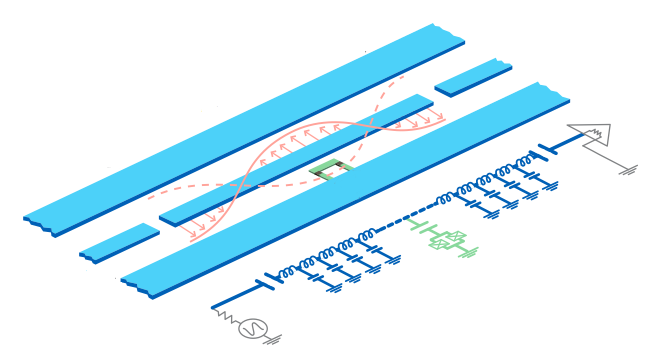
\includegraphics[width=3in]{SchustercQEDSchematic.png} 
   \caption[Schematic representation of cQED]{Schematic representation of cQED. Superconducting material (blue) is used for the resonator and ground planes. The center pin is shown with an oscillating electromagnetic wave (red). Capacitors couple the resonator to the input and output lines, containing the radiation within the cavity. The cavity is coupled to a nearby qubit (green), here placed in the dielectric gap near the center of the resonator. A circuit schematic is also shown. Figure modified from \cite{Schuster}.}
   \label{fig:cQEDSchematic}
\end{figure}

A one-dimensional transmission line acts as the cavity\footnote{The terms cavity, resonator, transmission line, and waveguide are used interchangeably.} within which photons propagate. The resonator is a conducting line separated from ground by a dielectric, as in a coaxial or fiber optic cable.The cavity resonant frequency is set by the length of the resonator between the two end capacitors.Typically, this is in the microwave regime\footnote{This is done to minimize thermal fluctuations affecting the circuit, as explained in Section \ref{sec:TransmissionLines}}. These capacitors act as mirrors, reflecting photons back and forth within the resonator. Vacuum conditions in the superconducting regime allow for remarkably low losses to be achieved.

Qubits are coupled to these transmission lines. To create quantum two-level systems, the typical electrical engineers toolbox is supplemented with the Josephson junction, the only known dissipationless non-linear circuit\cite{Devoret}. As shall be discussed in Section \ref{sec:Transmons}, a non-linear element is required to isolate two energy levels to serve as a computational qubit. Many different designs have been explored, in which different degrees of freedom operate as the computational basis states\footnote{For a good overview of possible superconducting qubit designs, see Ref. \cite{Clarke}.}. This is utilized for charge qubits such as the Cooper pair box\cite{Nakamura}, in which a charge difference between capacitors is created by the quantum tunneling of superconducting Cooper pairs. The conjugate variable to charge, flux, may also been used. By storing flux quanta in a superconducting loop, the persistent current (or number of flux quanta) becomes the basis states for a viable qubit. Quantum phase is also a possible variable for computation. Each qubit design has its own strengths and weaknesses, such as being sensitive to different types of noise. 

As in cavity QED, the composite qubit-resonator system reveals many interesting phenomena. Our chief method of realizing quantum information is via classical transmission measurements. By controlling the input and output of photons with the qubits, we can engineer ways to gain insight into the qubit states through familiar macroscopic parameters such as voltage and current. Typically, it is also possible to tune the qubit frequency into and out of resonance with the fixed cavity frequencies. Experiments, such as those in this thesis, rely on these two degrees of freedom. 

While this thesis does not explore any of the actual computational possibilities of the cQED architecture, multiple qubit-resonator buses may easily be coupled together to allow for the exchange and control of quantum information. CITE ARTICLE

%
%o	What is cQED: circuits based on cavity QED, ie. Realizing QED using superconducting circuits. 
%o	\cite{Blais} as starting the field
%o	“Electromagnetic signals are always composed of photons, although in the circuit domain those signals are carried as voltages and currents on wires, and the discreteness of the photon’s energy is usually not evident. However, by coupling a superconducting quantum bit to signals on a microwave transmission line, it is possible to construct an integrated circuit in which the presence or absence of even a single photon can have a dramatic effect.” \cite{Schuster Houck Resolving}
%o	Houck bullets
%•	Coupling qubits with photons
%•	Cavities enhance coupling, prevent information leakage
%•	Arbitrary pairwise coupling in one cavity
%•	Multiplexed readout and control
%o	Mirrored cavity suppresses decoherence
%o	Compress 2 dimensions of cavity to much less than a wavelength. This increases both the energy density and the dipole coupling. 
%o	\cite many papers, mention those that couple qubits together for actual computation (which I don’t cover)
%o	Low temperature → less thermal noise. If you think about the Boltzmann distribution, a really low temperature is required such that is prohibitively difficult to occupy the mode we are concerned with. At 20mK, the GHz regime corresponds to about 500mK, which is significantly greater



%Information is inherently a physical quantity, and the physics of information is the physics of all matter [Landauer1991]

\section{Outline}
Having given a brief introduction to quantum computing and cQED, this thesis continues in a much more focused manner. Chapter \ref{chap:Multimodal} presents the theoretical concepts investigated in this thesis: highly multimodal photon-qubit strong coupling in superconducting cQED circuits. While standard cQED operates typically couples the qubit only to the fundamental resonator frequency, it is theoretically possible to enter a new regime in which a qubit may \emph{simultaneously} couple to multiple modes of a cavity. We accomplish this by driving the resonator at high harmonics. To our knowledge, no work has been published in this field.  This thesis presents initial experimental work into the highly multimodal strong coupling regime. 


In order to understand these concepts, Chapter \ref{chap:Theoretical} presents an overview of topics standard to the literature. I feel it is most useful to understand the physics without getting too bogged down in the details of this particular thesis. As such, Chapter \ref{chap:Theoretical} is at a high level and should be applicable to any cQED system. I begin with the Jaynes-Cummings model as a prototypical cavity QED system, and explain the potential for this model to fit into the DiVincenzo criteria for quantum computing. From this, more advanced concepts are explored, such as nonlinear vacuum Rabi phenomena, cQED regimes, and more. 

Chapter \ref{chap:Multimodal} ETC

Chapter \ref{chap:Implementing} discusses the actual implementations of building superconducting circuits. An effort is made to justify the higher level theory of Chapters \ref{chap:Theoretical} and \ref{chap:Multimodal} as we build the physics of these circuits from the ground up. This chapter is also specific to this thesis, and focuses almost exclusively on the particular cQED designs used. It discusses coplanar waveguides, transmon qubits, and the physics of coupling the two. 

Finally, Chapter \ref{chap:Experimental} reveals the methods and results of this thesis. ETC



%%%%%%%%%%%%%%%%%%%%%%%%%%%%%%%%%%%%%%%%%%%%%%%%%%
\chapter{Theoretical basis of cQED}\label{chap:Theoretical}
This chapter presents the standard theory behind circuit quantum electrodynamics. My intention is for this introduction to be applicable to the field of cQED as a whole, regardless of the nuances of any particular implementation. As such, I will discuss certain concepts broadly; for example, while the all the circuits built for this thesis contained transmon qubits, this chapter will discuss how any viable qubit fits into the general cQED architecture. A specific discussion of the implementations used in this thesis can be found in Chapter \ref{chap:Implementing}. Familiarity with the concepts of this chapter is required to understand the novel theoretical and experimental work undertaken for this thesis, as found in Chapter \ref{chap:Multimodal}. Those readers comfortable with the cQED literature are invited to skip ahead. 

I begin with the abstract requirements for quantum computation, as laid out in the DiVincenzo criteria. This serves to explain how and why cQED is a viable quantum computing architecture. The Jaynes-Cummings model is then used as a starting point to conceptualize cQED. I will then delve into some more complicated, but standard, topics such as Vacuum Rabi phenomena and coupling regimes.

\section{Architectural objectives}\label{sec:DiVincenzo}
Quantum computing is motivated by a clear purpose: the manipulation and control of quantum information. For any physical system to be a viable quantum computer it must meet a stringent set of requirements, as first set out by David DiVincenzo \cite{DiVincenzo}:

\begin{enumerate}
\item A well-defined unit of quantum information, i.e. good qubits. Any two quantum energy levels can be used as a computational quantum states, and as such many implementations have been pursued. Importantly, qubits need not be an actual atom; there are macroscopic systems that can act as a quantum two-level system. 
\item Reliable state preparation. The ability to initialize qubits into a computational null state is a necessary starting point for performing any kind of meaningful computation.
\item Low decoherence. Maintaining quantum states of information is notoriously difficult, yet imperative.  A major challenge is to engineer sufficiently long qubit relaxation ($T_1$) and dephasing ($T_2$) times as compared to the time scale of computation. 
\item Accurate quantum gate operations. Qubits must be able to interact with another in a controlled manner. 
\item Quantum non-demolition  measurements, i.e. the ability to read out the state of the system without destroying any information. 
\end{enumerate}

Circuit quantum electrodynamics is just one implementation that seeks to satisfy the above criteria. The genius of cQED lies in the use of quantized electromagnetic radiation to solve (4) and (5). We place qubits satisfying (1) and (2) into a cavity. We then add photons to the cavity in a controlled manner\footnote{In addition, the high speed of photons eases the constraint on engineering (3).}. These photons may interact with the qubit states, either by modifying the qubit state (4) or by performing a non-demolition measurement of the system (5). Coupling cavities together allows for the interaction of qubits via photons. Cavities are the quantum bus of the cQED architecture. Such a system is described by the Jaynes-Cummings model, a common theoretical model in quantum optics. 



%%%%%%%%%%%%%%%%%%%%%%%%%%%%%%%%%%%%%%%%%%%%%%%%%%%%%%%%%%%%%%%%%%%%%%%%%
\section{Jaynes-Cummings model}\label{sec:JC}
The Jaynes-Cummings model describes a two-level quantum system coupled to the quantized mode of an optical cavity. This cavity may or may not contain photons. The simplest model in CQED, it was originally proposed to study light-matter interaction, specifically the phenomenon of spontaneous emission. As opposed to a semi-classical theory, the Jaynes-Cummings model allows for an understanding of how the discrete nature of electromagnetic radiation affects the system. As such, it is the ideal starting point from which to examine cQED. Fig. \ref{fig:ToycQED} presents a simplified visual diagram of the system.

\begin{figure}[h] 
   \centering
   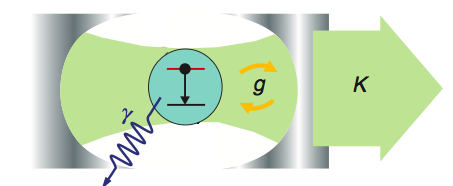
\includegraphics[width=3in]{Semba-Toy-cQED.png} 
   \caption[Jaynes Cummings model]{Jaynes-Cummings model. Green represents the EM field, blue represents the two-level quantum system and yellow the coupling between the two. The three rates $g$, $\kappa$ and $\gamma$ are schematically illustrated. In a cQED implementation, the cavity is replaced by a transmission line and the ``mirrors" shown are capacitors in the line. From \cite{Semba}.}
   \label{fig:ToycQED}
\end{figure}

Conceptually there are three main factors that describe the overall behavior of the system. First, the coupling between qubit and cavity modes is given by a rate constant $g$. This variable is dependent on numerous factors. Certain physical design considerations, such as the placement of the qubit in relation to the transmission line, are fixed for a particular circuit. As shall be mathematically described in Chapter \ref{sec:StrongCoupling}, the transition frequency of the qubit may be tuned in and out of resonance with the modes of the cavity. The tuning affects the coupling rate $g$. 

As no system is perfect, there are two main sources of decoherence. While we think of the walls of the cavity as ``mirrors," photons will leak out at a rate $\kappa$. Similarly, driving the addition of photons into the cavity is limited by the same rate. This term is determined by the engineering of the capacitors that enclose the resonator, as will be detailed in Chapter \ref{chap:Implementing}. 

The $\gamma$ term gives an all-encompassing rate for decoherence that may be experienced by the qubit. This relates directly to $T_1$ and $T_2$ times for the system; we can approximate $O(1/\gamma)= O(T_1,T_2)$. INCLUDE SPONTANEOUS EMISSION. As a qubit may be in a quantum superposition of states, it precesses, acting as a sort of clock measuring the frequency difference between the two states. If the qubit is subject to noise (internal or external) the clock can lose time or dephase, a subtle form of decoherence.\cite{Schuster} This form of decoherence occurs at the dephasing rate $T_2$.

Turning to the physics of the model, the Jaynes-Cummings Hamiltonian is given by

\begin{equation}\label{eq:JC}
H=\hbar \omega_r(a^\dag a + \frac{1}{2}) + \frac{1}{2}\hbar \omega_a \sigma_z + \hbar g(a^\dag \sigma_- + a\sigma_+)
\end{equation}

for a single cavity mode of frequency $\omega_r$.\footnote{The Jaynes-Cummings model is limited to describing a single photon mode. As in the cQED literature, this chapter defines the mode $\omega_r$ as the lowest harmonic of the cavity. } This follows the simplfied form

\begin{equation}
H_{\mathrm{JC}} = H_{\mathrm{field}}+H_{\mathrm{atom}}+H_{\mathrm{int}}.
\end{equation}

While it is imperative that the system be considered as a whole, I shall briefly describe the meaning of the three terms. Chapter \ref{chap:Implementing} will prove that the constituent parts of the cQED architecture are accurately described by these terms. 

%%%%%%%%%%%%%%%%%%%%%%%%%%%%%%%%%%%%%%%%%%%%%%%%%%
\subsection{Cavity modes}
Transmission lines in cQED act as quantized harmonic oscillators. As such, the possible frequencies of quantized EM radiation are dependent on the fundamental frequency of the cavity. These are closely related to integer multiples of twice the cavity length. This gives a linear spectrum of available frequencies. A quantized harmonic oscillator is described by 

\begin{equation}\label{eq:CavityHamiltonian}
H_{\mathrm{field}}=\hbar \sum_n\omega_n(a_n^\dag a_n+\frac{1}{2})
\end{equation}

for all possible frequencies. The raising and lowering operators work in the standard way

\begin{equation}
a^\dag\ket{n}=\sqrt{n+1}\ket{n+1} \hspace{1.3cm} a\ket{n}=\sqrt{n}\ket{n-1} 
\end{equation}

such that $a^\dag a\ket{n}=n\ket{n}$ reveals the number of photons in the cavity. However, we are often interested in the behavior of the circuit for one particular frequency. The case for the single resonant  frequency $\omega_r$ simplifies to 

\begin{equation}
H_{\mathrm{field}}=\hbar \omega_r(a^\dag a+\frac{1}{2}).
\end{equation}

As such, we define the state of the cavity by $\ket{n}$, $n \in \mathbb{Z}$, the number of photons of frequency $\omega_r$ in the cavity.

%%%%%%%%%%%%%%%%%%%%%%%%%%%%%%%%%%%%%%%%%%%%%%%%%%
\subsection{Qubit excitations}
As a two-level quantum system, the qubit has a ground state $\ket{g}$ and excited state $\ket{e}$. The transition energy $\hbar \omega_a$ between the two states is defined in terms of a frequency $\omega_a$. For the term $H_{\mathrm{atom}}$ to describe this physically we co-opt the two-dimensional Pauli inversion operator $\sigma_z$,

\begin{equation}
\sigma_z\ket{g}=-\ket{g} \hspace{1.3cm} \sigma_z\ket{e}=\ket{e}
\end{equation}

so that $H_{\mathrm{atom}}$ acting on the system gives eigenenergies $E_g=-\hbar\omega_a/2$ and $E_e=\hbar\omega_a/2$. The difference in energy between the two states is satisfied. 

%%%%%%%%%%%%%%%%%%%%%%%%%%%%%%%%%%%%%%%%%%%%%%%%%%
\subsection{Emission and absorption}\label{sec:Emission}
The qubit and cavity interact via dipole coupling. As a photon oscillates within the cavity, it produces an electric field. This electric field can cause an excitation of the qubit state. Considering conservation of energy, we can think of a photon being annihilated as energy is transferred from the cavity to the qubit. The shape of this electrical field depends on the cavity and frequency of the radiation; higher dipole moments occur at antinodes of the field. To increase coupling with a particularly frequency of radiation, it is important to place the qubit near one of these points.   

The final term $H_{\mathrm{int}}$, then, gives the energy of the dipole coupling between the qubit and cavity field.\footnote{This term is implicitly defined as being in the Rotating Wave approximation, which will be justified in Chapter \ref{chap:Implementing}.} The two possible interactions are the simultaneous annihilation of a photon and excitation of the qubit, $a\sigma_+$, as well as the inverse, $a^\dag \sigma_-$. We use the Pauli raising and lowering operators to describe the excitations of the qubit

\begin{eqnarray}
\sigma_+\ket{g} = \ket{e} \hspace{1.3cm} \sigma_-\ket{g} = \ket{0} \\
\sigma_+\ket{e} = 0\hspace{1.3cm} \sigma_-\ket{e} = \ket{g}. \nonumber
\end{eqnarray}

Note that the creation operator acting on the excited state, as well as the annihilation operator acting on theground state, produces $\ket{0}$. As expected, each subspace has only two distinct energy levels and therefore the coupling term $H_{\mathrm{int}}$ only connects the states $\ket{n,g}$ and $\ket{n-1,e}$.

By coupling the qubit and cavity modes there exist two tunable frequencies, $\omega_r$ of the cavity and $\omega_a$ of the qubit. Whether by engineering the length of the cavity to specific dimensions or tuning the qubit frequency $in$ $situ$, we can tune the frequencies into resonance with one another. This is defined by

\begin{equation}
\Delta = \omega_a - \omega_r.
\end{equation}

As stated in Chapter \ref{sec:JC}, the tuning parameter $\Delta$ affects the rate of coupling $g$. It also defines the regimes in which cQED can be operated, each of which gives rise to unique phenomena and can be used for different purposes. 

%%%%%%%%%%%%%%%%%%%%%%%%%%%%%%%%%%%%%%%%%%%%%%%%%%
\section{Quantum states}
With the Jaynes-Cummings model, we now understand how to parametrize the state of our system. A cQED circuit for a single cavity mode is described in two dimensions: (1) the qubit excitation state and (2) the number of photons in the cavity. We therefore describe the state of the entire system by a composite vector of the two subspaces. For example, the ground state of the entire system is given by $\ket{0,g}$, for which the qubit is in the ground state $g$ and there are no photons of the given frequency inside the cavity. 

By expressing the Jaynes-Cummings Hamiltonian (\ref{eq:JC})  in the basis of the excitation subsystems

\begin{equation}
\left(\begin{array}{cccccc} \ket{0,g} & \ket{1,g} & \ket{0,e} & ... & \ket{n, g} & \ket{n-1,e}
\end{array}\right).
\end{equation}

we can solve for the matrix representation

\begin{equation}\label{eq:Matrix}
H =  \hbar\left(\begin{array}{cccccccc}
0 \\
& \omega_r-\frac{\Delta}{2}	& g \\
& g    		& \omega_a-\frac{\Delta}{2} \\
&&&2\omega_r-\frac{\Delta}{2}	 & g\sqrt{2} \\
&&&g\sqrt{2}		& 2\omega_r + \frac{\Delta}{2}\\
&&&&&\ddots\\
&&&&&&n\omega_r-\frac{\Delta}{2} & g\sqrt{n}\\
&&&&&&g\sqrt{n}    & n\omega_r+\frac{\Delta}{2}
\end{array} \right)
\end{equation}

The coupling term causes the matrix to be block diagonal by only connecting the states $\ket{n,g}$ and $\ket{n-1,e}$. With the exception of the ground state, the 2-by-2 submatrix describing the $n^{th}$ excitation manifold is

\begin{equation}
\left(\begin{array}{cc}
\matrixel{n,g}{H}{n,g} & \matrixel{n-1,e}{H}{n,g} \\
\matrixel{n,g}{H}{n-1,e} & \matrixel{n-1,e}{H}{n-1,e}
\end{array}\right) = \hbar \left(\begin{array}{cc}
n\omega_r-\frac{1}{2}\Delta 	& g\sqrt{n} \\
 g\sqrt{n}					& n\omega_r+\frac{1}{2}\Delta
\end{array}\right)
\end{equation}

with yields the ``dressed" eigenstates\footnote{The variable $\theta_n$ satisfies $\tan{2\theta_n}=\frac{2g\sqrt{n}}{\Delta}$.} 

\begin{eqnarray}
\ket{n_+} &=& \sin(\theta_n)\ket{n,g}+\cos(\theta_n)\ket{n-1,e} \\
\ket{n_-} &=& \cos(\theta_n)\ket{n,g}-\sin(\theta_n)\ket{n-1,e}
\end{eqnarray}

with corresponding energies

\begin{eqnarray}
E_0/\hbar &=& -\frac{\Delta}{2} \\
E_n/\hbar &=& n\omega_r \pm \frac{1}{2}\sqrt{4ng^2+\Delta^2} .\nonumber
\end{eqnarray}

%As quantum computing is exceptionally sensitive to decoherence, any loss of information is a threat to maintaining quantum information. The strong coupling regime describes the ideal dynamics by which to solve such a problem. It is relatively easy for cQED architecture to realize this regime, a major reason this field is at the forefront of research into quantum computing. 

%%%%%%%%%%%%%%%%%%%%%%%%%%%%%%%%%%%%%%%%%%%%%%%%%%%%%%%%%%%%%%%%%%%%%%%
\section{Nonlinear Vacuum Rabi phenomena}\label{sec:Rabi}
Resonance, defined as tuning the cavity and resonator frequencies to be equal $\Delta=0$, leads to some truly remarkable phenomena in cQED systems. First, note that in the $\emph{uncoupled}$ resonant case $\omega_r=\omega_a$ the separate cavity and qubit systems both have a linear energy level spectrum $E_n=n\omega_{r,a}$, as expected for a simple harmonic oscilator. A transmission measurement of a bare cavity will reveal the linearity of the resonant frequencies, as modelled in Fig. \ref{fig:Transmission1}a. Resonance peaks are well described by the Lorentzian line shape

\begin{equation}
F_{\mathrm{Lor}}(\omega)=A_0\frac{\delta \omega}{(\omega-\omega_r)^2+\delta \omega^2/4}
\end{equation}

where $\delta \omega$ is the full width half maximum of the resonance. This relates to the quality factor $Q_L=\omega_r/\delta\omega$ of the resonator. 

\begin{figure}[h] 
   \centering
   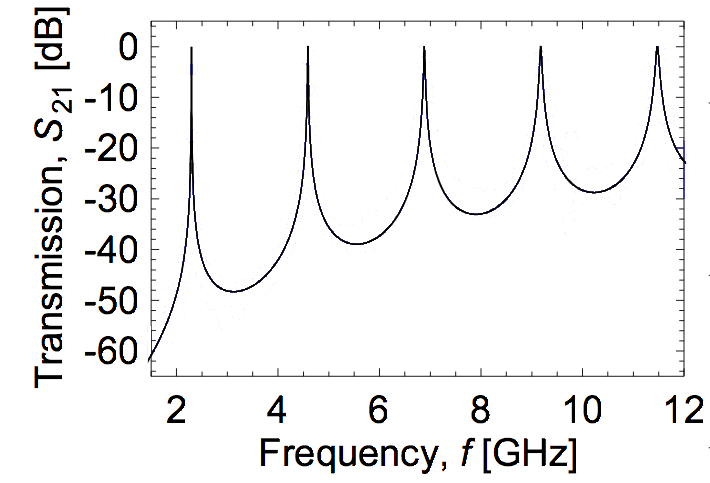
\includegraphics[width=2.5in]{Goppl-Higher-Modes.png} 
\includegraphics[width=2.5in]{placeholder.jpg} 
   \caption[Models of resonator transmission spectra]{Left: Model of the transmission spectrum of a bare cavity with $\omega_r=$2.3 GHz. Higher order harmonics are integer multiples of resonant frequency $\omega_r$. Each resonance peak clearly displays a Lorentzian lineshape. Figure is a best fit line of actual data taken from Ref. \cite{Goppl}. Right: Model of the transmission spectrum of a coupled cavity-qubit system at resonance. The ETC}
   \label{fig:Transmission1}
\end{figure}

However, resonance creates degeneracy in a coupled system. This can be observed by solving the Hamiltonian (\ref{eq:JC}) in the resonant limit. More specifically, so long $|\Delta|=|\omega_a-\omega_r|<<g$ we make the approximation $\omega_a=\omega_r$.\footnote{It's impossible for any lab setup to achieve perfection!} For a general subsystem of $n$ photons

\begin{equation}
H_n = \hbar \left( \begin{array}{cc}
n\omega_r & g\sqrt{n} \\
\sqrt{n}g & n\omega_r
\end{array}\right)
\end{equation}

we solve to find nonlinear energy eigenvalues

\begin{equation}\label{eq:NonlinearEnergies}
E_n = \hbar(n\omega_r\pm \sqrt{n}g)
\end{equation}

and simplified dressed eigenstates

\begin{equation}
\ket{n_{+,-}} = \frac{\ket{n,g}\pm\ket{n-1,e}}{\sqrt{2}}.
\end{equation}

Thus, coupling the atomic and cavity subsystems lifts the degeneracy by $2g\sqrt{n}$ at each energy level. a phenomena referred to as \emph{Vacuum Rabi splitting}. This creates an effective two-level system between the ground state $\ket{0,g}$ and antisymmetric eigenstate of the first excitation manifold $\ket{n_-}$, in which the transition energy between the two states is less than $\omega_r$. Fig. \ref{fig:EnergyLevels} shows both the degenerate and hybridized energy levels. 

\begin{figure}[h] 
   \centering
   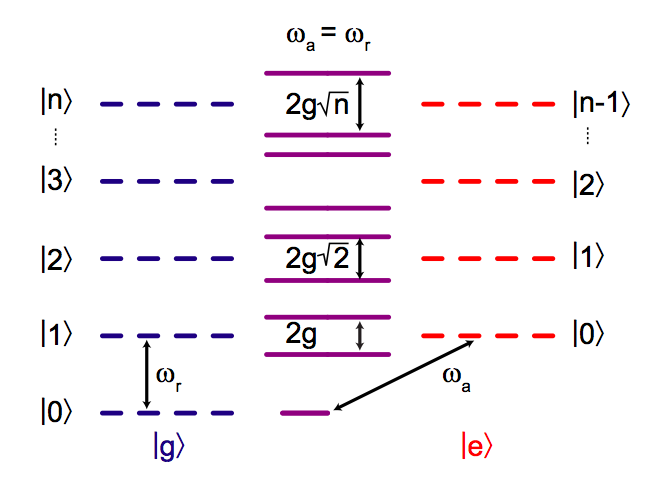
\includegraphics[width=3.5in]{SchusterResonantEnergyLevels.png} 
   \caption[Energy levels of JC Hamiltonian]{Energy level diagrams of the Jaynes-Cummings Hamiltonian. Energy levels for the uncoupled subsystems are shown using dotted lines, for both the qubit ground and excited states in blue and red, respectively. This diagram makes explicit the degeneracy of the uncoupled energy levels. A coupled system in the resonant strong coupling limit undergoes a nonlinear splitting of these levels by $2g\sqrt{n}$. From \cite{Schuster}.}
   \label{fig:EnergyLevels}
\end{figure}

A transmission measurement of the resonant, coupled system will show two transmission peaks around the resonant frequency $\omega_r$, one for each new eigenstate. Appropriately, this conveys the difference in eigenenergies, as the frequency splitting is $E_n/\hbar=2g\sqrt{n}$. PEAK WIDTHS? AFFECTS QUBIT STATE, HOW IS THIS DIFFERENT FROM DISPERSIVE MEASUREMENT?

In cQED the atom cannot be physically removed from the cavity to switch off the vacuum Rabi splitting —instead the atom is tuned far away from the cavity in frequency space. Vacuum Rabi splitting is thus typically observed in the form of an avoided crossing, occurring as the qubit frequency is tuned through resonance with the cavity\cite{Bishop}. Amazingly, at resonance the two frequencies $\omega_r$ and $\omega_a$ are never equal, despite the definition of resonance $\omega_r=\omega_a$. Coupling the system actually affects the modes of each individual subsystem. They will always differ by a frequency of at least $2\sqrt{n}g$. As $\Delta$ moves away from resonance, the states revert back to their unmixed form. An example of an avoided crossing is shown in Fig. (\ref{fig:AvoidedCrossing}).

\begin{figure}[h] 
   \centering
   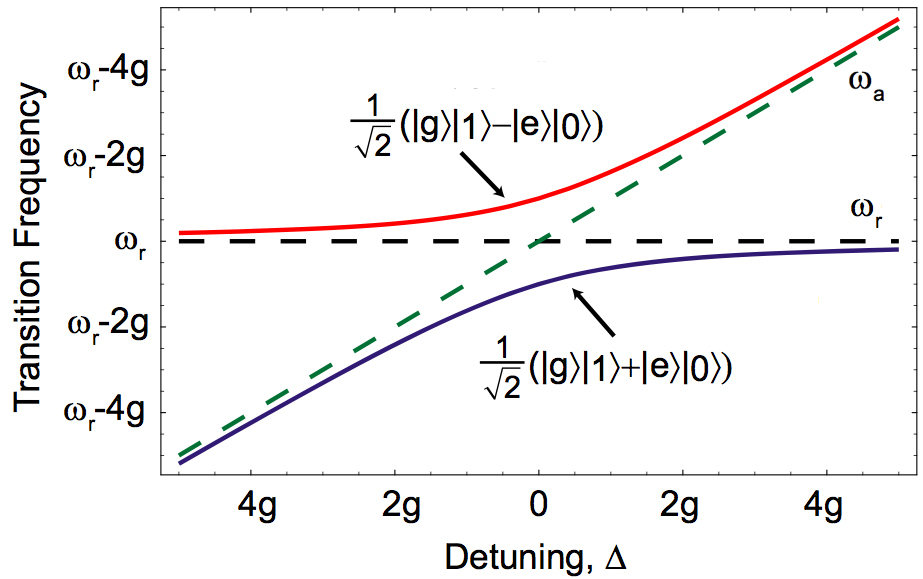
\includegraphics[width=4in]{SchusterAvoidedCrossing.png}%{ElizaAvoidedCrossing.png} 
   \caption[Model of vacuum Rabi splitting]{Model of an avoided crossing caused by vacuum Rabi splitting. The green and black dotted lines represent uncoupled $\omega_a$ and $\omega_r$, respectively. Resonance causes the coupled system to split into superposition eigenstates, shown in purple and red. The two superpositions are maximally split by 2$g$ at resonance. Far from resonance, these superpositions relax to the uncoupled states.}
   \label{fig:AvoidedCrossing}
\end{figure}

As the two eigenstates $\ket{n_+}$ and $\ket{n_-}$ differ in energy, the system will precess between the two states at the rate $2g\sqrt{n}$

\begin{equation}
\ket{\psi(t)}=\ket{n_-}+\ket{n_+}e^{i2\sqrt{n}gt}.
\end{equation}

Equivalently, this can be seen as an oscillation between our original basis states. Thus, any system placed in the pure state $\ket{n,g}$ will oscillate back and forth to $\ket{n-1,e}$. This oscillation between states is known as \emph{Vacuum Rabi oscillations}. 

%%%%%%%%%%%%%%%%%%%%%%%%%%%%%%%%%%%%%%%%%%%%%%%%%%%%%%%%%%%%%%%%%%%%
\section{Anharmonicity: Climbing the Jaynes-Cummings ladder}\label{sec:Anharmonicity}
Vacuum Rabi behavior is not proof of Jaynes-Cummings physics, as pointed out by Zhu \emph{et al.}\cite{Zhu} and Tian \emph{et al.}\cite{Tian}. Coupled classical harmonic oscillators can display the same hybridized mode splitting at resonant frequencies. However, resonant coupling also introduces a larger scale anharmonicity that is a uniquely quantum effect. Returning to  Eq. (\ref{eq:NonlinearEnergies}), energy levels at resonance are predicted to scale by the power law $n^{1/2}$ with the number of excitations $n$ of the system. This quantum effect is in stark contrast to the normal mode splitting of two classical couplied linear oscillators, which is independent of oscillator amplitude\cite{Fink}. This can be seen as a photon-photon interaction; introducing another photon to the system is dependent on the number of photons already in the cavity. This anharmonic behavior has been observed using Rydberg atoms in microwave cavities \cite{}, two-tone pump probe measurements \cite{Fink}, and for time-domain measurements of phase qubits \cite{Hofheinz, Wang}.
MORE? ANY DERIVATIONS?

%%%%%%%%%%%%%%%%%%%%%%%%%%%%%%%%%%%%%%%%%%%%%%%%%%%%%%%%%%%%%%%%
\section{cQED Regimes} %Or dispersive limit?
Circuit quantum electrodynamics can be characterized by a number of regimes. While this thesis is focused on effects seen in the strongly resonant limit, other regimes are of interest and necessary for experimental work. Typically, these regimes are determined by two parameters, strong vs. weak and resonant vs. dispersive (i.e. tuning $\Delta$). Fig. \ref{fig:Regimes} gives an overview of the parameter space. Note that I have already introduced vacuum Rabi behavior without first defining the strong coupling regime. While it is theoretically possible to achieve the resonant strong regime with a relatively small $g$ (by near perfect resonance), in practice cQED devices constructed for this purpose are also made to have high $g$ coupling. 

\begin{figure}[h] 
   \centering
   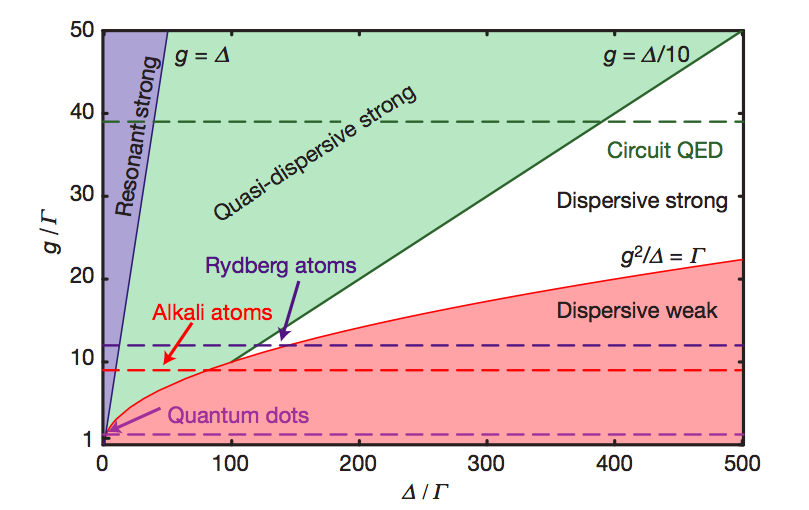
\includegraphics[width=4in]{HouckParameterSpace.png} 
   \caption[Parameter space diagram for cavity QED]{A parameter space diagram for cavity QED. The possible regimes are determined by the qubit-resonator coupling strength $g$ and resonance detuning $\Delta$. Each region is normalized by the rates of decay $\Gamma=\max[\gamma,\kappa,1/T]$. Possible regimes for cQED, Rydberg atoms, alkali atoms, and quantum dots are shown using dashed lines. Previously discussed vacuum Rabi behavior only occurs in the purple resonant strong regime. Fig. from \cite{SchusterResolving}.}
   \label{fig:Regimes}
\end{figure}

%%%%%%%%%%%%%%%%%%%%%%%%%%%%%%%%%%
\subsection{Strong coupling}\label{sec:StrongCoupling}
Strong coupling is defined as 

\begin{equation}
g>>[\gamma, \kappa]
\end{equation}

for which a single qubit can absorb and re-emit a single photon many times before decay. Recall that $g$ is the rate of coupling between the qubit and cavity. 

DOES THIS EXPLAIN INCREASING RATE OF COUPLING FOR EVERY PHOTON OSCILLATION, OR IS IT REALLY DECREASING DECOHERENCE??


%%%%%%%%%%%%%%%%%%%%%%%%%%%%%%%%%%
\subsection{Dispersive Limit}
Resonance has already been defined as $\Delta << g$; in the ideal case, $\Delta=0$. The dispersive limit is achieved by significant atom cavity detuning, $\Delta=|\omega_a-\omega_r| >> g$. Perturbation theory allows us to expand the Hamiltonian (\ref{eq:JC}) in powers of $g/\Delta$ to second order

\begin{eqnarray}
H&=&\hbar \omega_r\left(a^\dag a + \frac{1}{2}\right) + \frac{1}{2}\hbar \omega_a \sigma_z + \hbar g(a^\dag \sigma_- + a\sigma_+) \\
&\approx& \hbar\omega_r \left( a^\dag a +\frac{1}{2}\right)+\frac{1}{2}\hbar\sigma_z\left(\omega_a+\frac{2g^2}{\Delta}a^\dag a +\frac{g^2}{\Delta}\right) \label{eq:Dispersive}
\end{eqnarray}

which can be rewritten as 

\begin{equation}\label{eq:DispersiveQND}
H\approx \hbar\left( \omega_r+\frac{g^2}{\Delta}\sigma_z\right) \left(a^\dag a+\frac{1}{2}\right)+\frac{1}{2}\hbar\omega_a\sigma_z.
\end{equation}

Eqs. (\ref{eq:Dispersive}) and (\ref{eq:DispersiveQND}) are the same, yet they give different insights into the system. Eq. (\ref{eq:Dispersive}) maintains the nature of the cavity, instead highlighting a shift in the qubit's frequency. The qubit is modified by both a photon number-dependent ``Stark" shift ($2ng^2/\Delta$) and a vacuum noise induced ``Lamb" shift ($g^2/\Delta$). Physically when the atom state is changed it must electrically compress (or expand) the photons' wavelength, increasing (or decreasing) the frequency of each photon in the cavity, which will require extra energy ($\hbar g^2/\Delta$).

The equation is grouped to show the effect of the dispersive limit on the qubit's behavior. The qubit frequency undergoes a ``light" shift consisting of a photon number-dependent ``Stark" shift ($2ng^2/\Delta$) and a resonator vacuum induced ``Lamb" shift ($g^2/\Delta$)\cite{Schuster}. The latter shows the effect of coupling the subsystems even in the absence of excitations. The Stark shift term shows that, even in the dispersive limit, photon-qubit coupling will modify the state of the two-level system. 

Eq. (\ref{eq:DispersiveQND}) shifts focus onto the behavior of the resonator. The cavity experiences a frequency shift $\chi=g^2/\Delta$ dependent on the state of the qubit, $\sigma_z$. Thus, both the cavity and qubit experience frequency shifts subject to detuning by the power law $\Delta^{-1}$; this shows the gradual effects of tuning the qubit in and out of resonance\footnote{Note that this term only holds for the dispersive limit. In the resonant regime, $\Delta^{-1}$ does not apply, or else we'd have infinite frequency shifts!}. The energy levels of the system in the dispersive limit are shown in Fig. \ref{fig:DispersiveEnergyLevels}.

\begin{figure}[h] 
   \centering
   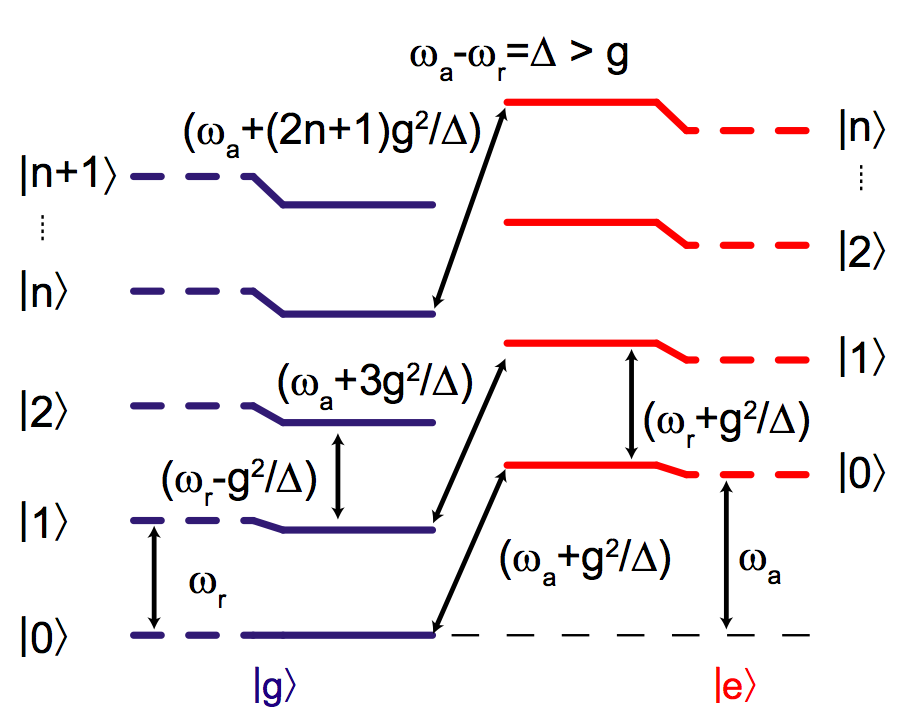
\includegraphics[width=3in]{SchusterDispersiveEnergyLevels.png} 
   \caption[Energy levels of JC Hamiltonian in the dispersive limit]{Energy levels of JC Hamiltonian in the dispersive limit ($\Delta\ll g$). The uncoupled energy levels of the system are depicted using dotted lines for $\omega_a > \omega_r$. In the coupled system, both the qubit and resonator experience frequency shifts proportional the perturbative term $g^2/\Delta$. The effective qubit frequency is $\omega_a'=\omega_a\pm(2n+1)g^2/\Delta$, for $n$ photons in the cavity. The effective cavity frequency is $\omega_r'=\omega_r\pm g^2/\Delta$. From \cite{Schuster}.}
   \label{fig:DispersiveEnergyLevels}
\end{figure}

The simultaneous dispersive shifts of both the qubit and resonator allows for Quantum non-demolition (QND) measurements in the strong limit, a necessary requirement from Chapter \ref{sec:DiVincezo}. Unlike in the resonant case, the frequency shifts for each subsystem are individual in nature, even if they are connected. A transmission measurement of resonant system will show the state of the qubit based upon the shift from $\omega_r$, however it acts as a direct measurement of the qubit and thus affects its state.

In the dispersive regime, the problem of determining the frequency of the qubit is rephrased to determining the bare resonator frequency (since this is different from any possible qubit frequency). For  Probing the system at this specific frequency, we can infer the state of the qubit! In the case that $\chi<\kappa$, multiple photons can be used to increase the gain of the measurement. As such, the dispersive regime is used for measurements of cQED systems. 

Conversely, measuring the state of the qubit will can provide information about the cavitys frequency. When the Stark shift $\chi$ exceeds the qubit decay $\gamma$, the qubit frequency is shifted by more than the linewidth of the transmission peak. As such, each individual photon mode is reflected in a distinct qubit frequency. While this is never computationally useful, it reflects a duality in the effects each of the two subsystems experiences. Fig. \ref{fig:DispersiveStrong} shows the behavior of all frequency shifts in the strong dispersive regime. 

\begin{figure}[h] 
   \centering
   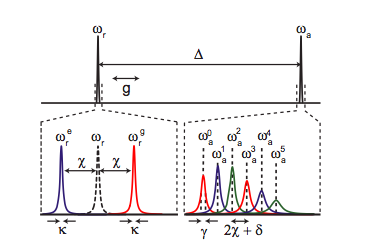
\includegraphics[width=3.5in]{SchusterDispersiveFrequencyShifts.png} 
   \caption[Transmission spectrum of coupled system in strong dispersive limit]{Transmission spectrum of coupled qubit-cavity system in strong dispersive limit. Top: Subsystems are far detuned by $\Delta$. Left: Resonator spectrum when the qubit is in the ground state (blue), excited state (red), or not present (dashed black). The width of the peaks is given by the ``leakage" of photons $\kappa$. Right: Qubit spectrum for different photon numbers in the cavity. The width of the peaks is given by the rate of qubit decoherence $\gamma$. Figure from \cite{Schuster}.}
   \label{fig:DispersiveFrequencyShifts}
\end{figure}

%%%%%%%%%%%%%%%%%%%%%%%%%%%%%%%%%%%%%%%%%%%%%%%%%%%%%%%%%%%%%%%%%%%%%%%%%%%%
%%%%%%%%%%%%%%%%%%%%%%%%%%%%%%%%%%%%%%%%%%%%%%%%%%%%%%%%%%%%%%%%%%%%%%%%%%%%
%%%%%%%%%%%%%%%%%%%%%%%%%%%%%%%%%%%%%%%%%%%%%%%%%%%%%%%%%%%%%%%%%%%%%%%%%%%%
\chapter{Highly multimodal photon-qubit strong coupling}\label{chap:Multimodal}

The current cQED literature has typically operated around the fundamental resonator frequency. This behavior is well described by the theory in Chapter \ref{chap:Theoretical}. However, we are interested in the possibility of higher harmonics opening up a new, multimodal regime. Recall that resonance in the strong coupling limit causes the system to split into superposition eigenstates, which themselves have an effective frequency difference of $2g\sqrt{n}$. Far from resonance, these superpositions relax back to the uncoupled eigenstates. By fabricating long resonators, it is possible to to create a device in which the fundamental frequency $\omega_0$ is on the order of the avoided crossing difference $2g\sqrt{n}$. Effectively, we are interested in the regime

\begin{equation}
\delta \omega \approx g
\end{equation}

for the mode splitting $\delta \omega \equiv \omega_n-\omega_{n-1}$.

Again beginning with the Jaynes-Cummings model, we can take into account the infinite series of harmonics $m$ above the fundamental frequency,

\begin{equation}
H_{MM}=\sum_{m=1}^M\left[\hbar m\omega_r (a^{\dag}_m a_m+\frac{1}{2})\right]+\hbar\omega_a\sigma_z+\sum^M_{m=1}\hbar g_m(a_m^+\sigma_-+a_m^-\sigma_+)
\end{equation}

Instead of simply describing the number of photons $\ket{n}$ of frequency $\omega_r$, we now expand our system to include the number of excitations of any harmonic mode by $\ket{m,n}$. For example, the ground state of the coupled system for the $m^{\mathrm{th}}$ harmonic is $\ket{m,0,g}$. 

Solving for the general manifold,

\begin{eqnarray}
\nonumber
\left(\begin{array}{cc}
\matrixel{m,n,g}{H}{m,n,g} & \matrixel{m,n-1,e}{H}{m,n,g} \\
\matrixel{m,n,g}{H}{m,n-1,e} & \matrixel{m,n-1,e}{H}{m,n-1,e}
\end{array}\right) 
\end{eqnarray}

yields the solution:

\begin{equation}\label{eq:GeneralSubmatrix}
\hbar \left(\begin{array}{cc}
m\omega_r\left(n+\frac{1}{2}\right)-\frac{\omega_a}{2}	& g_m\sqrt{n} \\
 g_m\sqrt{n}					& m\omega_r\left(n-\frac{1}{2}\right)+\frac{\omega_a}{2}
\end{array}\right).
\end{equation}

In order to examine the single excitation manifold of the multimodal system, we define the eigenstates

\begin{equation}
\left(\begin{array}{ccccccc} \ket{1,1,g} & \ket{1,0,e} & \ket{2,1,g} & \ket{2,0,e} & ... & \ket{m,1, g} & \ket{m,0,e}
\end{array}\right).
\end{equation}

This fixes $n=1$ for the general solution (\ref{eq:GeneralSubmatrix}). Examining the system at resonance with the fundamental frequency $\omega_r=\omega_a$,


\begin{equation}\label{eq:MultimodalMatrix}
H =  \hbar\left(\begin{array}{cccccccc}
\omega_r 	& g_1 \\
 g_1   		& \omega_r \\
&&\frac{5\omega_r}{2} & g_2 \\
&&g_2		& \frac{3\omega_r}{2}\\
&&&&\ddots\\
&&&&&\frac{(3m-1)\omega_r}{2}	& g_m \\
&&&&& g_m				& \frac{(m+1)\omega_r}{2}
\end{array} \right)
\end{equation}

we can solve for the eigenstates and eigenvalues of each mode $m$ for a single excitation, 

\begin{eqnarray}
v_{+,-}/\hbar = (-\frac{\omega_r-m \omega_r \pm \sqrt{4 g_m^2+\omega_r^2-2 m \omega_r^2+m^2 \omega_r^2)}}{2g_m}, 1) \\
E_{+,-}/\hbar = m\omega_r \pm\frac{1}{2}\sqrt{4 g_m^2+m^2 \omega_r^2-2 m \omega_r^2+\omega_r^2}.
\end{eqnarray}

Making the multimodal approximation $\delta \omega \approx g$, we can (very loosely) let $\omega_r\approx g_m$ for all $m$,

\begin{eqnarray}
E_{+,-}/\hbar  =m\omega_r  \pm \frac{\sqrt{\omega_r^2 m^2 -2 \omega_r^2 m+5 \omega_r^2}}{2}.
\end{eqnarray}

Coupling the system causes a splitting of the eigenvalues that scales approximately linearly with the mode number $m$.

IS THIS ACTUALLY HELPFUL / CORRECT?

To achieve the multimodal approximation, we are operating for modes around $m=100$. By this model, the energy level splitting is unreasonably large, in fact 50x larger than for the first mode.

?????????????????????????

%\begin{equation}\label{eq:MultimodalMatrix}
%H =  \hbar\left(\begin{array}{cccccccc}
%\omega_r 	& g_1 \\
% g_1   		& \omega_a \\
%&&\frac{6\omega_r-\omega_a}{2} & \sqrt{2}g_2 \\
%&&\sqrt{2}g_2		& \frac{2\omega_r+\omega_a}{2}\\
%&&&&\ddots\\
%&&&&&\frac{3m\omega_r-\omega_a}{2}	& g_m\sqrt{n} \\
%&&&&& g_m\sqrt{n}					& \frac{m\omega_r+\omega_a}{2}
%\end{array} \right)
%\end{equation}

%which yields the ``dressed" eigenstates\footnote{The variable $\theta_n$ satisfies $\tan{2\theta_n}=\frac{2g\sqrt{n}}{\Delta}$.} 
%
%\begin{eqnarray}
%\ket{n_+} &=& \sin(\theta_n)\ket{n,g}+\cos(\theta_n)\ket{n-1,e} \\
%\ket{n_-} &=& \cos(\theta_n)\ket{n,g}-\sin(\theta_n)\ket{n-1,e}
%\end{eqnarray}
%
%with corresponding energies
%
%\begin{eqnarray}
%E_0/\hbar &=& -\frac{\Delta}{2} \\
%E_n/\hbar &=& n\omega_r \pm \frac{1}{2}\sqrt{4ng^2+\Delta^2} .\nonumber
%\end{eqnarray}

%%%%%%%%%%%%%%%%%%%%%%%%%%%%%%%%%%%%%%%%%%%%%%%%%%%%%%%%%%%%%


%We expand the first excitation subsystem of the Jaynes-Cummings Hamiltonian (\ref{eq:Matrix}) to demonstrate new multimodal behavior
%
%\begin{equation}\label{eq:Matrix}
%H_1 =  \hbar\left(\begin{array}{cc}
%\omega_r 	& g \\
%g    		& \omega_a 
%\end{array} \right)
%\end{equation}
%
%The basis states are
%
%\begin{equation}
%\left(\begin{array}{cccccc} \ket{0,g} & \ket{1,g} & \ket{0,e} & ... & \ket{n, g} & \ket{n-1,e}
%\end{array}\right)
%\end{equation}
%
%The Jaynes-Cummings Hamiltonian has been implicitly been working with $n$ photons of frequency $\omega_r$. We now define $\omega_r$ to be the fundamental mode of the cavity, $m=1$. The variable $m$ will denote the harmonics of the modes for the quantum state. This differentiates between the second mode $m=2$ of a resonator of length $d$ and the fundamental mode $m=1$ for a resonator of length $d/2$, despite the two modes having the same frequency. This is necessary because the two resonators have drastically different mode spacings $\delta\omega_r$. 
%
%Having introduced the mode quantum number $m$, we write the quantum state of the system for the number of photons $n$ of mode $m$ for the fundamental resonator frequency $\omega_r$, with a qubit of transition frequency $\omega_a$ state $g$ or $e$
%
%\begin{equation}
%\ket{n,m,g} \hspace{0.7cm} \mathrm{or} \hspace{0.7cm} \ket{n,m,e}
%\end{equation}
%
%There is now a more complicated system of photon-qubit interaction. AT RESONANCE? In resonance, $\Delta=0$, there is still the regular method of qubit excitation/photon annihilation, and its inverse
%
%\begin{equation}
%\matrixel{n-1,e}{H}{n,g} =\matrixel{n,g}{H}{n-1,e} =\sqrt{n}g
%\end{equation}
%
%provided that the qubit frequency $\omega_a$ and the frequency of the photon causing the excitation are equivalent, i.e. the photon frequency is implicitly the fundamental mode $\omega_r$


%%%%%%%%%%%%%%%%%%%%%%%%%%%%%%%%%%%%%%%%%%%%%%%%%%%%%%%%%%%%%%%%%%%%%%%%%%%%
%%%%%%%%%%%%%%%%%%%%%%%%%%%%%%%%%%%%%%%%%%%%%%%%%%%%%%%%%%%%%%%%%%%%%%%%%%%%
%%%%%%%%%%%%%%%%%%%%%%%%%%%%%%%%%%%%%%%%%%%%%%%%%%%%%%%%%%%%%%%%%%%%%%%%%%%%
\chapter{Implementing cQED with superconducting circuits}\label{chap:Implementing}
Having discussed circuit quantum electrodynamics at a high level in Chapters \ref{chap:Theoretical} and \ref{chap:Multimodal}, we now turn to the engineering of such a system out of circuits. In discussing the physical implementation taken in this thesis, particular attention is paid to justifying the use of the Jaynes-Cummings model as a starting point for the previous chapters. The actual methods used to fabricate each device are discussed in Chapter \ref{chap:Experimental}.

The circuits designed for this thesis are, as compared to the field in general, relatively simple designs. They consist of a single extremely long transmission line resonator capacitively coupled to input and output lines. A single transmon qubit, an advanced form of a Cooper pair box charge qubit, is placed near the end of the resonator. These circuits are refrigerated and operated at approximately 20mK temperatures. As such, we first begin with some relevant theory on superconductivity. 

%%%%%%%%%%%%%%%%%%%%%%%%%%%%%%%%%%%%%%%%%%%%%%%%%%%%%%%%%%%%%%%%%%%%
\section{Superconductivity}
The theory of superconductivity is a vast subject, but I will give a brief treatment of areas relevant to superconducting circuits. Superconductivity is the quantum-mechanical phenomenon of zero DC resistance and the expulsion of magnetic fields (the Meissner effect) in certain materials when cooled below a critical temperature $T_c$. Niobium and aluminum, the two materials used for fabrication, have a critical temperature of 9.2 K and 1.2 K, respectively. This is easily reached by laboratory equipment, which can cool down to 20 mK.

BCS theory describes superconductivity as a microscopic effect caused by a condensation of pairs of electrons into a boson-like state. These pairs of electrons, called Cooper pairs, are correlated in momentum and spin, but not space. Cooper pairs form the basis of the Josephson junction, the nonlinear circuit element described in Section \ref{sec:Transmons}. As one electron moves in a superconducting material it will deform the lattice of nuclei. In response, another electron will adjust, lowering the total energy in response to the motion of the first. This can be rephrased as a pairing of electron-phonon interactions. As one electron emits a phonon, i.e. a quanta of lattice vibration, a second electron will absorb. Low temperatures are needed for this effect such that random thermal phonons do not interfere. 



%%%%%%%%%%%%%%%%%%%%%%%%%%%%%%%%%%%%%%%%%%%%%%%%%%%%%%%%%%%%%%%%%%%%
\section{Transmission lines}\label{sec:TransmissionLines}
Transmission lines form the resonators of the cQED architecture. Superconductors are used to minimize dissipative losses. The circuits in this thesis were constructed using niobium wafers on sapphire substrate.  More specific properties of the materials used are found in Section \ref{sec:CPW}. 

Certain design considerations must be taken in to account in building superconducting resonators. Current equipment will cool equipment  to approx. 20mK, i.e. $k_BT\approx2.76*10^{-28}$ joules. In considering potential sources of decoherence, it is important that the circuit (including the qubit) operate at a significantly higher energy scale than the thermal bath, or else random fluctuations are likely to destroy any coherent behavior. The higher end of the microwave spectrum, i.e. the GHz regime, corresponds to approx. 250mK temperatures, i.e. $k_BT\approx3.45*10^{-27}$. Using simple Boltzmann statistics, the potential for an unwanted transition due to thermal fluctuations is sufficiently negligible

\begin{equation}
e^{-\frac{3.45*10^{-27}}{2.76*10^{-28}}}=3.73*10^{-6}.
\end{equation}

Thus we can operate cQED in the microwave regime. Happily, our lab equipment allows for frequency sweeps from 4-11 GHz. This fixes the general length scales of the resonator. Using niobium, the minimum length of transmission line for a fundamental frequency of 4 GHz is approximately 1.5 cm. As we are ultimately interested in testing higher order harmonics, much longer resonators were actually fabricated. 

\begin{figure}[h] 
   \centering
   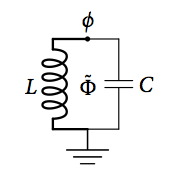
\includegraphics[height=3cm]{BishopLC.png} 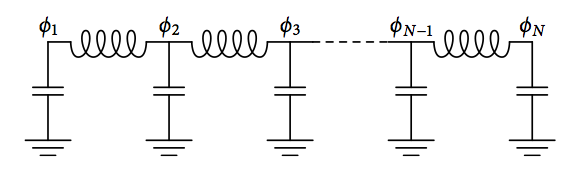
\includegraphics[height=3cm]{BishopLCChain.png} 
   \caption[LC oscillator]{Left: A simple LC oscillator, composed of an inductor $L$ and capacitor $C$ connected in a loop. Right: A transmission line resonator as an infinite chain of discrete LC oscillators. The inductors are coupled and capacitively connected to ground. Figures from \cite{Bishop}.}
   \label{fig:LCOscillator}
\end{figure}

To describe a quantized transmission line resonator, we begin with the textbook LC oscillator\footnote{Both \cite{Bishop} and \cite{Schuster}, being far better electrical engineers than I, also give a thorough treatment of the circuit from a classical starting point.}. This simple circuit, shown in Fig. \ref{fig:LCOscillator} consists of a inductor $L$ and capacitor $C$ connected in a loop. The circuit is used to store electrical energy oscillating at its resonant frequency. The inductor stores energy in its magnetic field, dependent on the current through the inductor. The voltage between the capacitor plates determines the energy stored in its electric field. Energy oscillates back and forth between the two units, creating an idealized dissipationless resonator. As we are operating at superconducting temperatures, we assume no resistance. The resonant frequency is determined by tuning the inductor and capacitor

\begin{equation}
\omega = \sqrt{\frac{1}{LC}}.
\end{equation}

As a resonator, the LC circuit has a quantum Hamiltonian identical in form to that of a simple harmonic oscillator. The two conjugate variables are the flux $\phi$ (from the inductor) and charge $q$ (from the capacitor)

\begin{equation}\label{eq:LCHamiltonian}
H=\frac{q^2}{2C}+\frac{\phi^2}{2L}.
\end{equation}

Defining the impedance as

\begin{equation}
Z=\sqrt{\frac{L}{C}}
\end{equation}

we can introduce creation and annihilation operators obeying 

\begin{eqnarray}
\phi=\sqrt{\frac{\hbar Z}{2}}\left(a+a^\dag\right) \\
q=-i\sqrt{\frac{\hbar}{2Z}}\left(a-a^\dag\right)
\end{eqnarray}

and the commutation relation $[a,a^\dag]=1$. This formulates the Hamiltonian (\ref{eq:LCHamiltonian}) as a measure of the excitations of the circuit

\begin{equation}\label{eq:SHO}
H=\hbar \omega\left(a^\dag a + \frac{1}{2}\right).
\end{equation}

The relationship between the canonical ``position" and ``momentum" variables is described by 

\begin{eqnarray}
\frac{\partial H}{\partial q}=\frac{q}{C}=-L\frac{\partial I}{\partial t}=-\dot{\phi} \label{eq:Hpartial}\\
\frac{\partial H}{\partial \phi}=\frac{\phi}{L}=I=\dot{q}.
\end{eqnarray}

A continuous chain of LC oscillators may be used to describe a transmission line beyond the lumped element approximation\cite{Pozar}. This is necessary for a circuits with dimensions on the same order as the electromagnetic wavelengths of interest. Following the derivation of \cite{Bishop}, we build a transmission line of length $d$, capacitance per unit length $c$ and inductance per unit length $l$. We use Eq. (\ref{eq:Hpartial}) to rewrite the Hamiltonian (\ref{eq:LCHamiltonian}) as a single-variable Lagrangian

\begin{equation}
L(\phi, \dot{\phi})=\frac{C\dot{\phi}^2}{2}-\frac{\phi^2}{2L}.
\end{equation}

%\begin{figure}[h] 
%   \centering
%   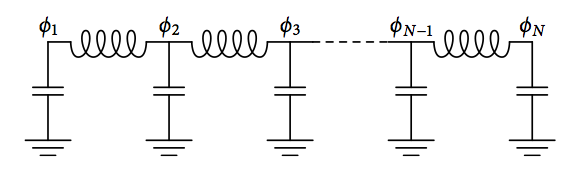
\includegraphics[width=3in]{BishopLCChain.png} 
%   \caption{A transmission line resonator as an infinite chain of discrete LC oscillators. Figures \cite{Bishop}.}
%   \label{fig:LCChain}
%\end{figure}

A chain of $N$ oscillators spanned by the inductor components, as seen in Fig. \ref{fig:LCOscillator} is described by  %figure used to be LCChain

\begin{equation}\label{eq:LCLagrangian}
L(\phi_1, \dot{\phi}_1,...,\phi_N, \dot{\phi}_N)=
\sum_{i=1}^N \frac{\Delta C \dot{\phi_i}^2}{2} -
\sum_{i=1}^{N-1}\frac{(\phi_{i+1}-\phi_i)^2}{2\Delta L}
\end{equation}

for which the capitance and inductance are broken down per unit length by $\Delta C=cd/N$ and $ld/N$, respectively. Letting $N\rightarrow \infty$, Eq. (\ref{eq:LCLagrangian}) becomes an integral over the length of the circuit

\begin{equation}\label{eq:LCLagrangianIntegral}
L[\phi(x,t),\dot{\phi}(x,t)]=
\int_0^d\frac{c\dot{\phi}(x,t)^2}{2}-\frac{1}{2l}\left(\frac{\partial\phi(x,t)}{\partial x}\right)^2\mathrm{d}x
\end{equation}

The corresponding Euler-Lagrange equation

\begin{equation}
\frac{\partial^2\phi}{\partial t^2}=v^2\frac{\partial^2\phi}{\partial^2 x}
\end{equation}

describes the dynamics of the circuit in the flux basis, revealing a wave velocity of $v=1/\sqrt{lc}$. The general solution is

\begin{equation}\label{eq:ELSolution}
\phi(x,t)=\sum_{n=1}^\infty A_n\cos(k_nx+\alpha_n)\cos(k_nvt+\beta_n)
\end{equation}

Open circuit boundary conditions are described by 

\begin{equation}
\frac{\partial\phi}{\partial x}\bigg|_{x=0}=\frac{\partial\phi}{\partial x}\bigg|_{x=d}=0
\end{equation}

which solves for $\alpha_n=0$ and the wave number $k_n=n\pi/d$. Combining this with the wave velocity, we find that our circuit has resonant frequency modes $\omega_n=nv\pi/d$. Substituting Eq. (\ref{eq:ELSolution}) into the Lagrangian (\ref{:LCLagrangianIntegral})  yields 

\begin{equation}
L(\Phi_1, \dot{\Phi_1})=\sum_{n=1}^\infty\frac{C_n\dot{\Phi_n}^2}{2}-\frac{\Phi_n^2}{2L_n}.
\end{equation}

$\Phi_n(t)=A_n\cos(k_nvt+\beta_n)$ is the final time-dependent solution, with effective capacitances $C_n=cd/2$ and inductances $L_n=2dl/n^2\pi^2$. Using the inverse of the original transform (\ref{eq:Hpartial}), we recover the quantum Hamiltonian for an extended transmission line resonator 

\begin{equation}
H=\hbar\sum_n \omega_n (a^\dag_n a_n + \frac{1}{2}).
\end{equation}

This Hamiltonian reflects the infinite, linear spectrum of mode frequencies that can exist in the cavity. Each individual mode behaves as a harmonic oscillator; the modification from (\ref{eq:SHO}) is the creation of a ladder of resonant modes.

 So far, our discussion of the circuit has been centered on the quantum variables $\phi$ and $q$. These terms describe the discrete nature of the possible electromagnetic excitations that may exist in the cavity. Remarkably, the resonator is sensitive to the existence of even a single photon. 

%%%%%%%%%%%%%%%%%%%%%%%%%%%%%%%%%%%%%%%%%
\subsection{Coplanar waveguide geometry}\label{sec:CPW}
$\kappa=2/RC$
$Q = \omega_0RC = \omega_0/\gamma$
This thesis used coplanar waveguide (CPW) geometry in constructing superconducting transmission line circuits. Chips were fabricated using 200 nm thick niobium coatings on sapphire ($\mathrm{Al_2O_3}$) substrate. The niobium center pin, input/output lines, and ground are all in the same plane. General CPW geometry is diagrammed in Fig. \ref{fig:CPW}. Table \ref{tab:CPW} lists the particular dimensions used in this thesis. 

\begin{table}[htb]
\centering
\begin{tabular}{|c|c|c|}
   \hline
   Dimension & Length ($\mu$m)\\
   \hline
   a & 10\\
   \hline
   s & 4.186\\
   \hline
   b & 18.372\\
   \hline
   t & 0.2\\
   \hline
   h & 500\\
   \hline
\end{tabular}
\caption[CPW geometries.]{CPW geometries for 1+1 finger capacitor designs. Variables correspond to dimensions shown in Fig. \ref{fig:CPW}. The two lengths $l$ correspond to the 10-by-10mm and 22-by-22mm chip designs, respectively. }
\label{tab:CPW}
\end{table} 

\begin{figure}[h] 
   \centering
   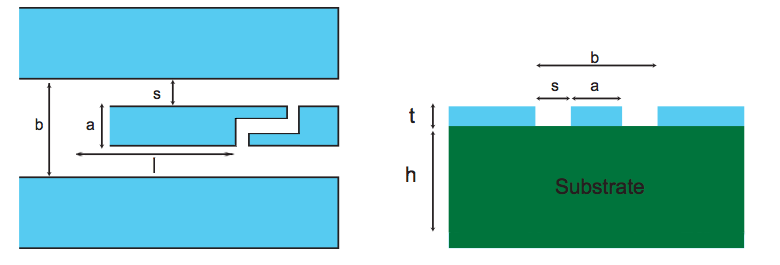
\includegraphics[width=4in]{SchusterCPW.png} 
   \caption[Coplanar waveguide geometry]{Coplanar waveguide geometry. Left: Top view of CPW resonator with 1+1 finger capacitor design. Length $l$ not to scale. The ratio $s/a$ determines the impedance $Z_0$. Resonator and ground plane (blue) are separated by a dielectric gap (white). Right: Cross section of CPW resonator fabricated on top of a substrate (green). The dielectric gap is vacuum. Figs. modified from \cite{Schuster}.}
   \label{fig:CPW}
\end{figure}

In experiment, multiple chip designs were tested. While the capacitor values listed in Table \ref{tab:CPW} are true for all devices, our initial tests of 1+1 finger capacitor designs had a low capacitance value of 1.56 fF. We therefore also built and tested 2+2 multi-finger design of the same dimensions. The increased capacitance (10.1fF) strengthened coupling. As a side note, the ground plane spacing of 4.186 $\mu$m was chosen to realize an impedance of 50 $\Omega$. 

Two chip sizes were design and tested: 10-by-10mm and 22-by-22mm. As the purpose of this thesis is to investigate highly multimodal behavior, chips were designed to maximize the length of the resonator\footnote{I initially experimented with coplanar waveguide thicknesses of 10 $\mu$m and 20 $\mu$m, before only 10 $\mu$m were ever cooled down for experiments. Due to space constraints as well as the possibility for greater multimodal behavior in the longer 10 $\mu$m thickness devices, the thicker waveguide design was abandoned.}. To maintain ``linearity" in the waveguide, curvature in the line was constrained to a radius of 180 $\mu$m (in the center of the line). Each chip also had a 1mm border to ensure safety from scratches and defects in the fabrication process. These were the two primary constraints on the possible length of the devices. 

The length of each device determines the resonance spectrum of the device. The first mode $l=1$ has a wavelength $\lambda=2l$, i.e. the lowest harmonic has a node in the center of the resonator. The entire spectrum is described by integer multiples ($n \in \mathbb{Z}$) of the resonant frequency, 

\begin{equation}
\nu=\frac{c}{\sqrt\epsilon_{\mathrm{eff}}}\frac{n}{2l}
\end{equation}

The effective dielectric permittivity is a function of the waveguide width, ground plane spacing, substrate thickness, and relative permittivity of the substrate. For all chips, these dimensions and the materials were held constant, such that $\epsilon_{\mathrm{eff}}=5.15$ and $v_{\mathrm{ph}}=c/\sqrt\epsilon_{\mathrm{eff}}\approx 132,000,000$ m/s. For the various resonator lengths used, Table (\ref{tab:ResonanceSpectrum}) gives the fundamental harmonic mode as well as all the modes in the relevant 4-11 GHz microwave range. As you can see, we have attempted to operate at exceptionally high harmonics. 

\begin{table}[htb]
\centering
\begin{tabular}{|c|c|c|c|}
   \hline
   Chip design & Length (m) & $f_0$ (MHz) & GHz modes ($l$) \\
   \hline
   10mm, 1+1 finger & 0.363 & 181.678 & 22-60\\
   \hline
   10mm, 2+2 finger & 0.364 & 181.785 & 22-60\\
   \hline
   22mm 1+1 finger & 2.229 & 29.648 	& 136-371 \\
   \hline
\end{tabular}
\caption[Chip modes]{Chip modes. The harmonic modes in the relevant 4-11 GHz range are given in the last column. Typically, only the fundamental mode is utilized.}
\label{tab:ResonanceSpectrum}
\end{table} 

%\begin{table}[htb]
%\centering
%\begin{tabular}{|c|c|c|}
%   \hline
%   Chip design & Length (m) & Cap. (fF)\\
%   \hline
%   10mm, 1+1 finger & 0.363 & 1.56\\
%   \hline
%   10mm, 2+2 finger & 0.364 & 10.1\\
%   \hline
%   22mm 1+1 finger & 2.229 & 1.56\\
%   \hline
%\end{tabular}
%\caption[]{}
%\label{tab:CPW}
%\end{table} 

%%%%%%%%%

We used transmission matrix analysis, more commonly known as ABCD matrices, to characterize CPW transmission spectra near resonance. A symmetrically coupled resonator is defined by the product of an input-, a transmission-, and an output matrix as 

\begin{equation}
\left(\begin{array}{cc}
A & B \\
C & D
\end{array}\right) 
=\left(\begin{array}{cc}
1 & Z_{\mathrm{in}} \\
0 & 1
\end{array}\right) 
\left(\begin{array}{cc}
t_{11} & t_{12} \\
t_{21} & t_{22}
\end{array}\right) 
\left(\begin{array}{cc}
1 & Z_{\mathrm{out}} \\
0 & 1
\end{array}\right) 
\end{equation}

with input/output impedances $Z_{\mathrm{in/out}}=1/i\omega C_\kappa$ and the transmission matrix parameters\cite{Goppl}

\begin{eqnarray}
t_{11} &=& \cosh(\gamma l) \\
t_{12} &=& Z_0\sinh(\gamma l) \\
t_{21} &=& 1/Z_0\sinh(\gamma l) \\
t_{22} &=& \cosh(\gamma l).
\end{eqnarray}

The wave propagation coefficient $\gamma=\alpha+i\beta$ is a function of the attenutation constant $\alpha=Z_0/Rl$ and the phase constant $\beta=\omega_n/v_{\mathrm{ph}}$. HOW TO CALC ATTENUATION CONSTANT

%%%%%%%%%%%%%%%%%%%%%%%%%%%%%%%%%%%%%%%%%%%%%%%%%%%%%%%%%%%%%%%%%%%%
\section{Superconducting qubits}\label{sec:SuperconductingQubits}
As discussed in Section \ref{sec:DiVincenzo}, the qubit is designed to be a two-level system. I have already shown that quantized harmonic oscillators have a infinite, linear spectrum of energy levels. It is therefore impossible to isolate any two energy levels as computational basis states such that driving a transition between these two levels will not also populate other, erroneous energy levels. 

A two-level quantum system is achieved by introducing anharmonicity. While an anharmonic circuit is not strictly two-level, as many energy levels exist, a good superconducting qubit is designed to have sufficient anharmonicity such that it is effectively two-level within a specific frequency range. The Josephson junction\cite{Devoret2004}, the only known dissipationless nonlinear circuit, is used in many superconducting qubit designs, including the transmon. 
%%%%%%%%%%%%%%%%%%%%%%%%%%%%%%%%%%%%%%
\subsection{Josephson junction}

The Josephson junction is consists of two superconductors with a very thin insulating layer (approx. 10 atoms) in between. This is also known as a superconductor-insulator-superconductor junction (SIS). Cooper pairs tunneling between the junctions cause a small oscillatory current $I(t)$. Ref. \cite{Tinkham} derives the relationship to the branch flux across the junction,

\begin{equation}
I(t)=I_0\sin\left(\frac{\phi(t)}{\phi_0}\right)
\end{equation}

in which $I_0$ is the critical current and $\varphi$ the gauge invariant phase difference between the two superconducting islands. The magnetic flux quantum $\phi_0=\hbar/2e$ directly relates to the charge of a single Cooper pair. The nonlinear inductive behavior of the junction is apparent in the sinusoidally time-dependent term. 

We can use the above relation to find the potential energy stored in the Cooper pairs that have tunneled across the junction:

\begin{equation}
E(t)=\int V(t)I(t)dt = I_0\int_{-\infty}^{t}    \dot{\phi}\sin\left(\frac{\phi(t)}{\phi_0}\right)=
-E_J\cos\left(\frac{\phi(t)}{\phi_0}\right)+\mathrm{const}.
\end{equation}

The Josephson energy of the junction is defined as $E_J=I_0\phi_0$.


%%%%%%%%%%%%%%%%%%%%%%%%%%%%%%%
\subsection{Transmons}\label{sec:Transmons}
The transmission-line shunted plasma oscillation qubit\cite{Koch}, otherwise known as the \emph{transmon}, was used for this thesis. The circuit design, modified from the Cooper pair box\cite{Bouchiat, Nakamura}, consists of two superconducting islands coupled by two Josephson junctions\footnote{Two Josephson junctions may be connected in parallel to form a single effective junction.}. The charge operator $n=-q/2e$ measures the difference between the islands in units of the Cooper pair charge $2e$. Due to this discreteness, the behavior of the Josephson element is periodic in flux $-E_J\cos((2e/\hbar)\phi)$. 

IS GATE VOLTAGE OR FLUX THE FLUX BIAS LINE? WHAT IS PHI?

The circuit is surprisingly simple, as seen in Fig. \ref{fig:TransmonCoupling}, replacing the inductor in the quantized harmonic oscillator of Eq. (\ref{eq:SHO}) with two Josephon junctions in parallel. The Hamiltonian is

\begin{equation}
H=\frac{q^2}{2C}-E_J\cos\left(   \frac{2e}{\hbar}\phi     \right)
\end{equation}

which can be in the standard form

\begin{equation}\label{eq:TransmonHamiltonian}
H=4E_C(n-n_g)^2-E_J\cos\varphi
\end{equation}

using identities for the charging energy $E_C=e^2/2C$ and gauge invariant phase $\varphi=(2e/\hbar)\phi$. The charge offset $n_g=Q_r/2e+CgVg/2e$ arises from the DC voltage $V_g$ of the flux bias line (gate) or charges from any other stray couplings $Q_g$. Appendix B of Ref. \cite{Koch}  solves for the eigenenergies in terms of Mathieu functions

\begin{equation}
E_m(n_g)=E_C a_{2[n_g+k(m,n_g)]}(-E_J/2E_C)
\end{equation}

in which $a_\nu(q)$ denotes Mathieu's characteristic value and $k(m, n_g)$ is a function for sorting eigenvalues. 


The Hamiltonian, then, clearly depends on the ratio of the Josephson and charging energies $E_J/E_C$ as well as the effective offset charge $n_g$. Fig. \ref{fig:KochEigenenergies} plots the eigenvalues for various energy ratios. Two things are immediately noticeable. First, anharmonicity of qubit is inversely proportional to the ratio $E_J/E_C$. Second, the eigenenergies flatten with increasing $E_J/E_C$. The transmon is tuned to operate in the regime $E_J\gg E_C$, i.e. with relatively little anharmonicity but stable eigenvalues. 

We can better understand this by introducing the \emph{charge dispersion}, $\epsilon_m$, defined as the peak-to-peak energy range for the $m^{\mathrm{th}}$ eigenvalue as $n_g$ is varied

\begin{equation}\label{eq:ChargeDispersion}
\epsilon_m \equiv E_m(n_g=1/2)-E_m(n_g=0).
\end{equation}

\begin{figure}[h] 
   \centering
   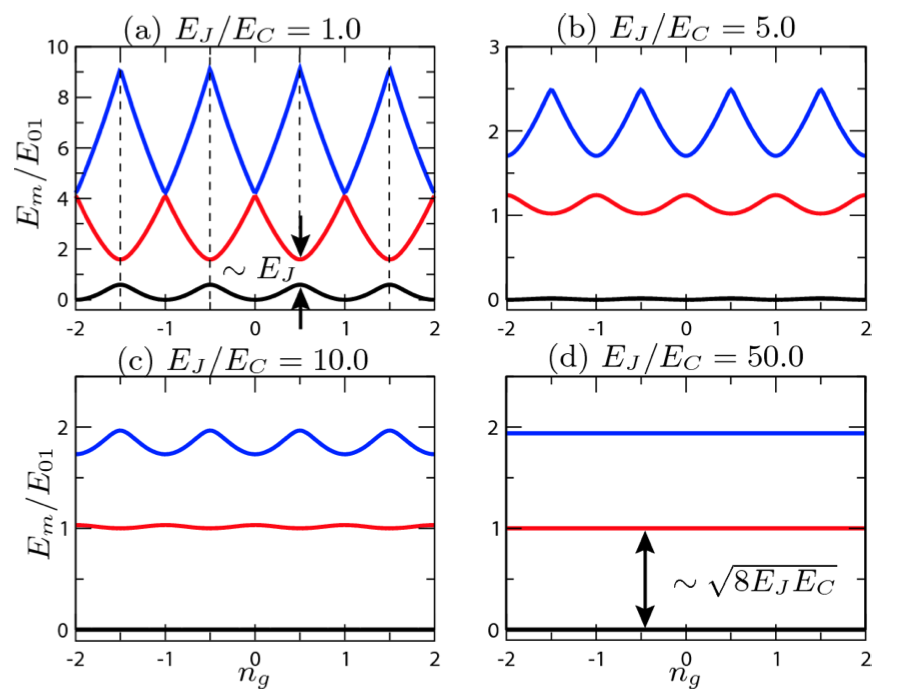
\includegraphics[width=5in]{Koch-Transmon-eigenenergies.png} 
   \caption[Transmon eigenenergies and charge dispersion]{Transmon eigenenergies and charge dispersion. At low $E_J/E_C$ the eigenenergies are parabolic functions of $n_g$ with avoided crossings. As $E_J/E_C$ increases, charge dispersion decreases exponentially until the eigenvalues are constant. The anharmonicity between neighboring eigenenergies only decreases algebraically. Figures from \cite{Koch}.}
   \label{fig:KochEigenenergies}
\end{figure}

For large $E_J/E_C$, the dispersion relation is well-approximated by

\begin{equation}
E_m(n_g)\approx E_m(n_g=1/2)-\frac{\epsilon_m}{2}\cos(2\pi n_g).
\end{equation}

While Eq. (\ref{eq:ChargeDispersion}) is the exact definition of $\epsilon_m$, Ref. \cite{Koch} used WKB methods to solve for the asymptotic behavior of the charge dispersion for $E_J/E_C\gg 1$. The resulting expression

\begin{equation}
\epsilon_m\approx(-1)^m E_C \frac{2^{4m+5}}{m!}\sqrt{\frac{2}{\pi}}\left(\frac{E_J}{2E_C} \right)^{\frac{m}{2}+\frac{3}{4}}e^{-\sqrt{8E_J/E_C}}
\end{equation}

reveals the crucial exponential decrease of the charge dispersion with $\sqrt{E_J/E_C}$.

The strength of this qubit design is revealed by comparing the exponential behavior of the charge dispersion relation to the anharmonic behavior of the transmon. As $E_J\gg E_C$, we can expand the Hamiltonian (\ref{eq:TransmonHamiltonian}) to fourth order

\begin{equation}
H=4E_Cn^2-E_J +\frac{E_J\varphi^2}{2}-\frac{E_J\varphi^4}{24}.
\end{equation}
 
The $n_g$ dependence is removed as in the transmon regime the qubit experiences only exponentially small charge dispersion. Identifying the quadratic terms as a harmonic oscillator, we can define standard  creation $z^{\dag}$ and annihilation $z$ operators such that 

\begin{equation}
H=-E_J+\sqrt{8E_CE_J}(z^{\dag}z+1/2)-\frac{E_C}{12}(z^{\dag}+z)^4.
\end{equation}

As the transmon only has weak anharmonicity, we can approximate the left-over quartic term by perturbation theory, yielding eigenenergies

\begin{equation}\label{eq:PerturbationAnharmonicity}
E_m\cong-E_J+\sqrt{8E_CE_J}\left( m+\frac{1}{2}\right)-\frac{E_C}{12}(6m^2+6m+3).
\end{equation}

Defining\footnote{Definitions of anharmonicity are modified from Ref. \cite{Koch} to consider anharmonicity of higher energy states.} the absolute anharmonicity of the transmon as 

\begin{equation}
\alpha_m \equiv E_{m,m+1}-E_{m-1,m}
\end{equation}

Eq. (\ref{eq:PerturbationAnharmonicity}) reveals the asymptotic behavior

\begin{equation}
\lim_{m\rightarrow\infty}\alpha_m =-E_C.
\end{equation}

We can compare this absolute anharmonicity to the lowest transition energy $E_{01}=\sqrt{8E_JE_C}$ of the transmon

\begin{equation}
\alpha_m^r = \alpha/E_{01}\cong-(8E_J/E_C)^{-1/2}.
\end{equation}

This is the relative anharmonicity, showing that the anharmonicity only decreases $algebraically$ with $E_J/E_C$.

Returning to the charge dispersion, the two relations proven in this section demonstrate that operating the transmon at large $E_J/E_C$ will exponentially reduce charge noise sensitivity while only sacrificing a small amount of anharmonicity. A typical example, taken from Ref. \cite{Bishop}: a transmon with energy ratio $E_J/E_C=60$ and transition frequency $E_01/\hbar=5$ GHz has anharmonicity of 271 MHz and charge dispersion of 1.8 kHz. 

%
%o	\cite{Koch}: 
%o	Intro: 
%•	Def: “a transmission-line shunted plasma oscillation qubit”. “The transmon consists of two superconducting islands coupled through two Josephson junctions, but isolated from the rest of the circuitry.” Currently the most promising candidate for a scalable quantum computing architecture. 
%•	“A promising physical paradigm for quantum computers is the superconducting Josephson junction qubit [5,6,7], which is classified into three types according to their relevant degree of freedom: charge [8,9], flux [10,11], and phase[12].”
%•	Based off Cooper Pair Box
%•	Advantages: 
%•	“Designed to operate in a regime of significantly increased ratio of Josephson energy and charging energy E_J/E_C. “
%•	Charge dispersion: “the variation of the energy levels with respect to environmental offset charge and gate voltage, and determines the sensitivity of the CPB to charge noise
%•	photo and electron beam lithography
%•	“The charge dispersion reduces \exponentially in EJ/EC, while the anharmonicity only decreases \algebraically by slow power law”
%•	cite{Koch} Figs 1 and 2
%•	But there are many other types of (superconducting) qubits: flux, charge, and phase.  See Table 1.1 in \Schuster for qubits
%o	How to build Transmon
%•	Josephson junctions
%•	Nonlinearity→anharmonicity. Needed to realize discrete nature of photons. 
%•	“The Josephson junction consists of two superconductors separated by an insulating layer thin enough so that Cooper pairs can tunnel through it. There is then a phase difference \delta=\phi_1-\phi_2 in the Cooper pair condensates across the 
%•	CPB
%•	\cite{Devoret}, \cite{Nakamura}
%•	Two Josephson junctions. WHAT IS JOSEPHSON ENERGY?
%•	Charge qubit, based on Cooper Pair tunneling. The qubit state is the charge difference between the islands. 
%•	“This large energy density, together with the large geometric capacitance (dipole moment) of the CPB, yields an interaction strength that is g/\omega_{a,r}=2% of the total photon energy…maintaining g/\gamma_{eff}=40 possible coherent vacuum Rabi oscillations in the strong resonant regime, where \gamma_{eff}=(\gamma+\kappa)/2 is the combined photon-qubit decay rate” \cite{Schuster Houck Resolving}
%•	“This dc-SQUID setup allows for the tuning of the Josephson energy…by means of an external magnetic flux \phi”
%•	Transmon, \cite{Koch}
%•	Difference from CPB: “a shunting connection of the two superconductors via a large capacitance C_B, accompanied by a similar increase in the gate capacitance C_g”
%•	“Designed to operate in a regime of significantly increased ratio of Josephson energy and charging energy E_J/E_C. “ ie, order of several tens to several hundreds
%•	Q factor of 10^7 and 0.3ms relaxation time (for 8GHz). Spontaneous emission?
%•	Charge dispersion?
%•	“The gate voltage V_g across the gap creates an electromagnetic field around the Cooper pair box, which has a dipole moment resulting from the charge difference between its two superconducting islands A voltage between the islands V_j results and is a fraction \beta of V_g; \beta is called the voltage division of the circuit and is, as we shall see, a dimensionless quantity linearly related to the setups coupling strength g.”\cite{Eliza}
%Clarke: The development of more advanced charge qubits such as the transmon20 and quantronium12 has greatly ameliorated this problem. The transmon is a small Cooper- pair box that is made relatively insensitive to charge by shunting the Josephson junction with a large external capacitor to increase Ec and by increasing the gate capacitor to the same size. Consequently, the energy bands of the type shown in Fig. 3c are almost flat, and the eigenstates are a combination of many Cooper-pair-box charge states. For reasons that will be discussed later (see the section ‘Decoherence’), the transmon is thus insensitive to low-frequency charge noise at all operating points. At the same time, the large gate capacitor provides strong coupling to external microwaves even at the level of a single photon, greatly increas- ing the coupling for circuit quantum electrodynamics (QED) (see the section ‘Quantum optics on a chip’).


%%%%%%%%%%%%%%%%%%%%%%%%%%%%%%%%%%%%%%%%%%%%%%%%%%%%%%%%%%%%%%%%%%%%
\section{Cavity-Qubit coupling}
Embedding a transmon qubit into a superconducting transmission line realizes the cQED architecture. The transmon is placed in close proximity to the coplanar waveguide. This connects the two circuits via a dipole coupling from the oscillating electromagnetic field of the photons in the transmission line. As the transmission line is capacitively coupled to ground (as well as input and output lines), the ends of the line are appoximated as antinode maxima of the electric field. To maximize dipole interaction, the qubit should be placed at an antinode; typically the center of the transmission line is chosen, coupling to the second harmonic, $l=2$ of the cavity, as seen in Fig. \ref{fig:TransmonCoupling}b. 

WE DON"T DO THIS

\begin{figure}[h] 
   \centering
   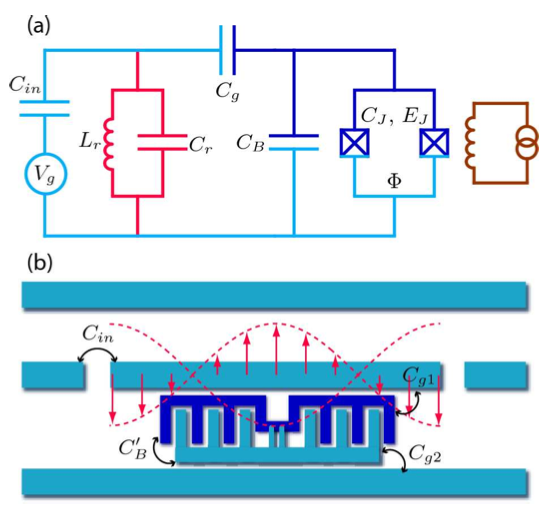
\includegraphics[height=3in]{KochTransmon.png} 
   \caption[Transmon circuit schematic]{(a) Effective circuit diagram of the transmon qubit (dark blue), resonator (red), flux biasing circuit (brown) and voltage-biasing circuit (cyan, not used in this thesis TRUE?). (b) Schematic drawing, not to scale. The transmon consists of two superconducting islands acting as multidigit capacitors (one dark blue, one teal) shunted by a short section of twin-lead transmission line. The resonator is shown with an $l=2$ mode oscillating electromagnetic wave. Figures from \cite{Koch}.}
   \label{fig:TransmonCoupling}
\end{figure}

The Hamiltonian is the sum of the transmon Hamiltonian (\ref{eq:TransmonHamiltonian}) and transmission line Hamiltonian (\ref{eq:SHO}), as well as a dipole coupling term,

\begin{equation}\label{eq:CQC}
H=4E_C(n-n_g)^2-E_J\cos(\varphi)+\hbar\omega_ra^{\dag}a+2\beta eV^0_{\mathrm{rms}}n(a+a^{\dag}).
\end{equation}

The coupling term is proportional to both the charge of the transmon $n$ and the quantized electric field $(a+a^{\dag})$ in the resonator. Detailed calculations are worked out in Appendix A of Ref. \cite{Koch}.

It is useful to write the above Hamiltonian in terms of the uncoupled transmon states $\ket{i}$. By this nomenclature the transmon terms simplify to $\hbar\sum_j\omega_j\ket{j}\bra{j}$. Defining the coupling strength $g$ by

\begin{equation}
\hbar g_{ij}=\beta\bra{i}n\ket{j}
\end{equation}

we can rewrite the Hamiltonian (\ref{eq:CQC}) as

\begin{equation}\label{eq:CQC2}
H=\hbar\sum_j\omega_j\ket{j}\bra{j}+\hbar\omega_r\left(a^{\dag}a+\frac{1}{2}\right)+\hbar\sum_{i,j}g_{ij}\ket{i}\bra{j}(a+a^{\dag})
\end{equation}

around the transmission line resonant frequency $\omega_r$. Treating the transmon as an effective two-level system, we make define the identities $\ket{0}\rightarrow\ket{\downarrow}$ and and ignore higher order transmon states. The Hamiltonian (\ref{eq:CQC2}) for the coupled system then further simplifies to

\begin{equation}
H=\frac{1}{2}\hbar\omega_a\sigma_z+\hbar\omega_r\left(a^{\dag}a+\frac{1}{2}\right)+\hbar g\sigma_x(a+a^{\dag}).
\end{equation}

The final step is the so-called rotating wave approximation

\begin{equation}
\sigma_x(a+a^{\dag})=a^{\dag}\sigma_- + a\sigma_+.
\end{equation}

This ignores the terms $a\sigma_-$ and $a^{\dag}\sigma_+$, neither of which conserve the number of excitations in the coupled system. The resulting expression is the famous Jaynes-Cummings Hamiltonian 

\begin{equation}
H=\hbar \omega_r\left(a^\dag a + \frac{1}{2}\right) + \frac{1}{2}\hbar \omega_a \sigma_z + \hbar g(a^\dag \sigma_- + a\sigma_+)
\end{equation}

used as the starting point for Chapter \ref{chap:Theoretical}. 

%%%%%%%%%%%%%%%%%%%%%%%%%%%%%%%%%%%%%%%%%%%%%%%%%%
\section{Fabrication procedures}
The fabrication process is long, time-consuming, and fraught with opportunity to make mistakes. Considering the large surface area used for each chip, it was especially difficult to fabricate without any defects, such as scratches, shorts, photoresist debris, etc. 

\subsection{Masks}
Masks were designed in AutoCAD 2011 and printed using optical lithography. Our masks were soda-lime  with a 530 nm layer of AZ1518 photoresist . A Heidelberg DWL-66 laser lithography system 405nm UV light with 40mW was used with a 4mm focal length writehead, providing minimum feature sizes of about 0.8 $\mu$m. TYPE OF MASK. This was then developed with an AZ400K dilution (1:4 with water) using a Laurell Technology Corporation Spin Processor EDC650Mz. Masks were etched with CR-7 chrome etchant and subsequently cleaned in PRS-1000. 

\subsection{Photolithography}
Wafers are 200 nm niobium coatings on sapphire substrate. Niobium is a superconductor with critical temperature 9.2 K.  below After dicing and cleaning, wafers are spun with HMDS and AZ5214 photoresist before being baked at 105$^o$ C for 2 minutes. The HMDS acts an adhesive for the photoresist. 

Photolithography was performed with a Karl Suss MJB4 Mask Aligner. The MJB4 uses broad spectrum light from a mercury lamp for the exposure illumination. Each wafer was exposed to the mask pattern for 4 seconds before being developed in AZ300MIF for approximately 1 minute. The mask pattern exposes the inverse of the coplanar waveguide geometry. This niobium will be removed during the etching process, i.e. the dielectric gaps will be removed. The vast majority of the niobium, constituting the center pin and ground plane, remains. 

\subsection{Etching}
Dry etching was performed with an STS OTHER NAME? EXPLAIN DRY ETCH

\begin{figure}[h] 
   \centering
   
\includegraphics[width=2in]{placeholder.jpg} 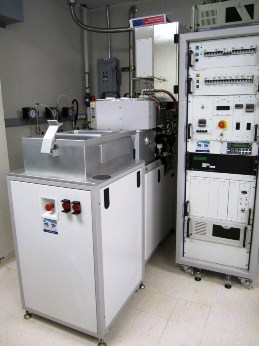
\includegraphics[width=2in]{STS.jpg} 
   \caption[Photolithography and etching tools]{Photolithography and etching tools. Left: Karl Suss MJB4 mask aligner used for photolithography. Right: STS ?????}
   \label{fig:Wirebonding}
\end{figure}

\subsection{Packaging}
After being etched, each wafer must be diced to the exact dimensions of device. This allows for the chip to fit into fridge mounts, shown in Fig. \ref{fig:Mounts}. The wafers are coated with AZ4330 photoresist to protect them during the dicing process. Dicing was done with an ADT proVectus 7100 using a hubless resin blade. 

At this point, we used electron beam lithography to fabricate qubits on some of the devices. Some devices were left without qubits to measure the transmission spectrum of the resonator without any interference. It is also a time intensive process to perform e-beam lithography and, as it is the only device I was not authorized to use, the decision to fabricate qubits was made sparingly.

The final packaging process is mounting and wirebonding the chip. The copper bond pads were meticulously cleaned with water, a fiber optic pen to remove rust, flux, and isopropanol. Silver paste was used as the adhesive to fix the chip onto the bond pad. The chip design was aligned to the 6 input/output lines on the bond pad.

Extensive wirebonding accomplished a few purposes. Thankfully, we had a new Questar Automatic Wire Bonder to help. First, the three coplanar waveguide connections on the chip were connected to three different input/output lines on the copper bond pad. Second, the ground plane of the chip was extensively wirebound to the body of the bond pad. This provides a stronger path to ground. Both connections are shown in see Fig. \ref{fig:Wirebonding}a. Finally, we wirebound across the dielectric gap of each turn in the transmission line, see Fig. \ref{fig:Wirebonding}b. The nature of the design meant that one ``side" of the ground plane (with respect to the center pin) had a stronger connection to ground. Connecting both sides of the ground plane balances this out. 

\begin{figure}[h] 
   \centering
   
\includegraphics[width=2in]{placeholder.jpg} 
\includegraphics[width=2in]{placeholder.jpg} 
   \caption[Applications of wire bonding]{Applications of wire bonding. Left: wire bonds attach the input/output lines of the bond pad to the resonator and flux bias lines of the chip. All around the outsde of the chip, the superconducting ground plane is attached to copper on the bond pad. Right: wire bonds equilibrate the superconducting ground plane on either side of the dielectric gap.}
   \label{fig:Wirebonding}
\end{figure}

Our lab contains two fridges NAMES, the typical chip size of which is 10mm-by-10mm. We also chose to design a 22mm-by-22mm chip, which necessitated building a custom mounting plate, shown in Fig. (\ref{fig:CustomMount})

\subsection{Electron beam lithography}
The necessary feature size of our transmon is on the order of 100 nm, too small for optical lithography. Instead, all transmon qubits were fabricated using electron beam lithography. The initial mask design left a 40-by-300 $\mu$m dielectric gap 700 $\mu$m from one capacitive end of the resonator. The transmon is thus fabricated directly onto the sapphire substrate. 

A bilayer resist system was used, in which both chemicals are sensitive to electrons rather than UV light. The bottom layer of MMA (ethyl-lactate 13$\%$) is spun to a thickness of approximately 550 nm. On top of this we add a 120 nm thick layer of PMMA. As MMA is the more sensitive of the two, a natural undercut will occur which aids in the creating the three-dimensional features needed from the liftoff step. Finally, a 12 nm layer of aluminum is added on top. This is to avoid charging and to give the electrons a ground plane; as the layer is so thin, exposure to any area will still develop the photoresist, especially at the high voltages used in the actual lithographic writing process. We used a Raith e-Line electron beam lithography tool, see Fig. \ref{fig:Raith}. 

\begin{figure}[h] 
   \centering
   \includegraphics[width=3in]{RaitheLine.jpg} 
   \caption[Raith e-Line]{Raith e-Line electron beam lithography tool.}
   \label{fig:Raith}
\end{figure}

After exposure, DEVELOP PROCESS IN LAB ASK SRI


%%%%%%%%%%%%%%%%%%%%%%%%%%%%%%%%%%%%%%%%%%%%%%%%%%%%%%%%%%%%%%%%%%%%%%%%%%%%
%%%%%%%%%%%%%%%%%%%%%%%%%%%%%%%%%%%%%%%%%%%%%%%%%%%%%%%%%%%%%%%%%%%%%%%%%%%%
%%%%%%%%%%%%%%%%%%%%%%%%%%%%%%%%%%%%%%%%%%%%%%%%%%%%%%%%%%%%%%%%%%%%%%%%%%%%
\chapter{Experimental methods and results}\label{chap:Experimental}


%%%%%%%%%%%%%%%%%%%%%%%%%%%%%%%%%%%%%%%%%%%%%%%%%%%%%%%%%%%%%%%%%%%%%%%%%%%%
%%%%%%%%%%%%%%%%%%%%%%%%%%%%%%%%%%%%%%%%%%%%%%%%%%%%%%%%%%%%%%%%%%%%%%%%%%%%
%%%%%%%%%%%%%%%%%%%%%%%%%%%%%%%%%%%%%%%%%%%%%%%%%%%%%%%%%%%%%%%%%%%%%%%%%%%%
\newpage
\bibliography{ThesisBib}
\bibliographystyle{ieeetr}

%\nocite{*}


\end{document}